\documentclass[11pt,a4paper]{article}
\usepackage[T1]{fontenc}
\usepackage[utf8]{inputenc}
\usepackage{lmodern,microtype}
\usepackage[margin=25mm]{geometry}
\usepackage{amsmath,amssymb,bm,graphicx,booktabs,tabularx,longtable,array}
\usepackage[font=small,labelfont=bf]{caption}
\usepackage{enumitem,placeins,xurl}
\usepackage[numbers,sort&compress]{natbib}
\usepackage[colorlinks=true,allcolors=blue,breaklinks=true]{hyperref}
\usepackage{doi}
\hypersetup{pdftitle={Extending Fisher-KPP glioma growth with oxygen and necrosis: simulation and synthetic parameter recovery},pdfauthor={}}
\setlength{\emergencystretch}{2em}
\setlength{\parskip}{3pt}
\setlist{nosep,leftmargin=*}
\newcolumntype{Y}{>{\raggedright\arraybackslash}X}
\newcommand{\pos}[1]{\left[#1\right]_{+}}
\newcommand{\dd}{\mathrm{d}}
% Generated by make_figures.py; do not edit.
\newcommand{\CoupledCells}{2.426}
\newcommand{\ReferenceCells}{2.847}
\newcommand{\CellReduction}{14.80}
\newcommand{\VolumeReduction}{1.85}
\newcommand{\CoupledVolume}{48.832}
\newcommand{\ReferenceVolume}{49.752}
\newcommand{\CoupledPeak}{0.637}
\newcommand{\ReferencePeak}{0.896}
\newcommand{\NecroticCells}{2.930}
\newcommand{\NecroticVolume}{0.024}
\newcommand{\MinimumOxygen}{0.0804}
\newcommand{\MaximumNecrosis}{1.226}
\newcommand{\NativeMinimumOxygen}{0.0513}
\newcommand{\NativeMaximumNecrosis}{3.416}
\newcommand{\NativeCellReduction}{14.78}
\newcommand{\CellGapMillion}{421.24}
\newcommand{\BirthGapMillion}{418.31}
\newcommand{\ZeroUptakeError}{6.64e-07}
\newcommand{\TestCount}{50}

\newcommand{\AblationRows}{%
M0: Fisher--KPP & 2.847 & 49.752 & 1.944 & --- & --- \\
M1: oxygen-limited growth & 2.429 & 48.856 & 0.000 & 0.0962 & 0.000 \\
M2: oxygen and necrosis & 2.426 & 48.832 & 0.000 & 0.0804 & 2.930 \\
M2, fixed supply ($\alpha=0$) & 2.829 & 49.744 & 0.976 & 0.2245 & 0.000 \\
M2, zero uptake ($\beta=0$) & 2.847 & 49.752 & 1.944 & 1.0000 & 0.000 \\
}

\newcommand{\RefinementRows}{%
2 & 0.25 & 2.4258 & 2.9302 & 0.0804 & 1.226 \\
2 & 0.125 & 2.4239 & 2.9431 & 0.0798 & 1.266 \\
2 & 0.0625 & 2.4230 & 2.9493 & 0.0795 & 1.285 \\
1 & 0.125 & 2.4524 & 3.6067 & 0.0513 & 3.416 \\
}

\newcommand{\ErrorRows}{%
0.25 & 0.1270 & 0.0129 & 4.238 \\
0.125 & 0.0423 & 0.0043 & 1.386 \\
}

% Generated from outputs/synthetic_recovery; do not edit.
\newcommand{\RecoveryDTrue}{0.300}
\newcommand{\RecoveryRhoTrue}{0.045}
\newcommand{\RecoveryDEstimate}{0.3033}
\newcommand{\RecoveryRhoEstimate}{0.04510}
\newcommand{\RecoveryDRelativeError}{+1.09}
\newcommand{\RecoveryRhoRelativeError}{+0.22}
\newcommand{\RecoveryBootstraps}{100}
\newcommand{\RecoveryTrials}{60}
\newcommand{\RecoveryDCoverageCount}{59}
\newcommand{\RecoveryRhoCoverageCount}{60}
\newcommand{\RecoveryCorrelation}{+0.540}
\newcommand{\RecoveryDayNinetyRMSE}{$8.42\times10^{-4}$}
\newcommand{\RecoveryDayNinetyGridRMSE}{$3.41\times10^{-4}$}
\newcommand{\RecoveryDayNinetyTimeRMSE}{$6.19\times10^{-5}$}

\newcommand{\RecoveryRows}{%
$D$ (mm$^2$/day) & 0.30000 & 0.30326 & [0.27217, 0.33791] & [0.27257, 0.33507] \\
$\rho$ (day$^{-1}$) & 0.04500 & 0.04510 & [0.04413, 0.04609] & [0.04430, 0.04604] \\
}

\newcommand{\RecoveryCoverageRows}{%
$D$ (mm$^2$/day) & $+2.64\times10^{-3}$ & $1.71\times10^{-2}$ & 59/60 (98.3\%) & [91.1, 100.0]\% \\
$\rho$ (day$^{-1}$) & $+3.60\times10^{-7}$ & $4.48\times10^{-4}$ & 60/60 (100.0\%) & [94.0, 100.0]\% \\
}

\newcommand{\RecoveryForecastRows}{%
75 & $4.72\times10^{-4}$ & 0.03036 & 94.0\% \\
90 & $8.42\times10^{-4}$ & 0.03018 & 94.6\% \\
}

% Generated from outputs/brainweb_recovery; do not edit.
\newcommand{\BWBootstraps}{100}
\newcommand{\BWTrials}{60}
\newcommand{\BWWhiteEstimate}{0.49806}
\newcommand{\BWGrayEstimate}{0.08264}
\newcommand{\BWRhoEstimate}{0.03948}
\newcommand{\BWWhiteError}{-0.39}
\newcommand{\BWGrayError}{-17.36}
\newcommand{\BWRhoError}{-1.30}
\newcommand{\BWWhiteCoverage}{57}
\newcommand{\BWGrayCoverage}{55}
\newcommand{\BWRhoCoverage}{59}
\newcommand{\BWCorrelation}{-0.582}
\newcommand{\BWCondition}{35.14}
\newcommand{\BWDayNinetyRMSE}{$3.72\times10^{-3}$}
\newcommand{\BWNearDayNinetyRMSE}{$7.30\times10^{-3}$}
\newcommand{\BWDayNinetyGridRMSE}{$3.68\times10^{-3}$}
\newcommand{\BWDayNinetyTimeRMSE}{$1.50\times10^{-4}$}
\newcommand{\BWHalfTimeRMSE}{$5.01\times10^{-5}$}
\newcommand{\BWGrayStressEstimate}{0.114350}
\newcommand{\BWGrayStressShift}{14.35}

\newcommand{\BWRecoveryRows}{%
$D_{\rm WM}$ (mm$^2$/day) & 0.50000 & 0.49806 & [0.45121, 0.54978] & [0.45033, 0.54892] \\
$D_{\rm GM}$ (mm$^2$/day) & 0.10000 & 0.08264 & [0.05714, 0.11952] & [0.05543, 0.10749] \\
$\rho$ (day$^{-1}$) & 0.04000 & 0.03948 & [0.03899, 0.03997] & [0.03886, 0.03992] \\
}

\newcommand{\BWCoverageRows}{%
$D_{\rm WM}$ (mm$^2$/day) & $+2.21\times10^{-3}$ & $2.44\times10^{-2}$ & 57/60 (95.0\%) & [86.1, 99.0]\% \\
$D_{\rm GM}$ (mm$^2$/day) & $+1.10\times10^{-3}$ & $1.86\times10^{-2}$ & 55/60 (91.7\%) & [81.6, 97.2]\% \\
$\rho$ (day$^{-1}$) & $-1.13\times10^{-5}$ & $2.06\times10^{-4}$ & 59/60 (98.3\%) & [91.1, 100.0]\% \\
}

\newcommand{\BWForecastRows}{%
75 & Full FOV & 0.00227 & 0.02004 & 94.9\% \\
75 & Near seed & 0.00496 & 0.02056 & 95.0\% \\
90 & Full FOV & 0.00372 & 0.02064 & 94.2\% \\
90 & Near seed & 0.00730 & 0.02344 & 89.2\% \\
}

\newcommand{\BWAnatomyRows}{%
$D_{\rm WM}$ (mm$^2$/day) & 0.50000 & 0.500218 & +0.04\% & 0.499160 \\
$D_{\rm GM}$ (mm$^2$/day) & 0.10000 & 0.114350 & +14.35\% & 0.096770 \\
$\rho$ (day$^{-1}$) & 0.04000 & 0.039948 & -0.13\% & 0.039445 \\
}

\title{Extending Fisher--KPP glioma growth with oxygen and necrosis:\\a reproducible BrainWeb simulation and synthetic parameter recovery study}
\author{}
\date{Working manuscript --- 17 October 2026}
\begin{document}
\maketitle
\begin{abstract}
\noindent\textbf{Background.} Fisher--Kolmogorov--Petrovskii--Piskunov (Fisher--KPP) models describe glioma spread and growth but do not explicitly represent oxygen limitation or necrotic material. We developed a minimal coupled extension and an interactive workflow to examine these assumptions.\par
\noindent\textbf{Methods.} Tissue-dependent Fisher--KPP, oxygen-limited growth and viable-tumor--oxygen--necrosis dynamics were compared on BrainWeb over 90 days with assigned biological parameters. Analytical checks, ablations and refinement assessed the numerical method. Two synthetic experiments estimated homogeneous diffusion/proliferation and separate white-/gray-matter diffusion with shared proliferation from blurred, voxel-averaged signals. Early scans calibrated each fit; later scans were withheld. Each experiment used 100 bootstrap fits and 60 independent noise trials. BrainWeb inference additionally tested a change in anatomy/grid resolution.\par
\noindent\textbf{Results.} On the 2 mm forward grid, coupling reduced day-90 viable count by \CellReduction\% versus Fisher--KPP, while low-threshold volume differed by \VolumeReduction\%. Growth inhibition dominated; localized necrosis and oxygen minima remained grid sensitive. Homogeneous rates were recovered within bootstrap 95\% intervals. In BrainWeb, known rates $(D_{\rm WM},D_{\rm GM},\rho)=(0.5,0.1,0.04)$ were estimated as $(\BWWhiteEstimate,\BWGrayEstimate,\BWRhoEstimate)$ in mm$^2$/day, mm$^2$/day and day$^{-1}$. The true proliferation rate fell just outside both 95\% intervals in the primary realization. Independent local-interval coverage was \BWWhiteCoverage/\BWTrials{}, \BWGrayCoverage/\BWTrials{} and \BWRhoCoverage/\BWTrials{}, respectively. Fitting noise-free 2 mm anatomy with the 3 mm model shifted gray-matter diffusion by +\BWGrayStressShift\%.\par
\noindent\textbf{Conclusions.} Oxygen feedback can alter the modeled interior despite similar threshold-defined extent. Conditional two- and three-rate inference is feasible under known initialization and imaging assumptions, but noise-based intervals omit anatomy/discretization error. Translation requires calibrated observation operators, broader uncertainty assessment, independent biological targets and external forecasts.
\end{abstract}
\noindent\textbf{Keywords:} glioma; reaction--diffusion; oxygen; necrosis; BrainWeb; parameter identifiability; MRI; validation.
\section{Introduction}
Reaction--diffusion models describe an expanding population through spatial dispersal and local growth. The Fisher--KPP equation emerged from Fisher and from Kolmogorov, Petrovskii and Piskunov \citep{fisher1937,kpp1937}. Related proliferation--invasion formulations describe glioma-cell migration through anatomically heterogeneous brain tissue. Distinguishing white- and gray-matter motility permits predictions of preferential spread even when local transport is isotropic \citep{swanson2000}.

A single viable-cell field omits microenvironmental processes that can distinguish an infiltrating margin from a poorly oxygenated interior. The histological illustration motivating this work, from Comba et al., emphasizes invasion routes, vascular niches, reactive cells and necrosis \citep{comba2021}; the present model represents only a small subset of that conceptual picture. Earlier mechanistic modeling connected oxygen, cellular phenotypes and necrosis to pseudopalisading patterns \citep{martinez2012}. Our reduction does not reproduce that model or explicitly resolve pseudopalisades. Oxygen-dependent proliferation and transfer into a necrotic compartment introduce additional assumptions and parameters. A more elaborate model can reproduce more patterns without providing uniquely identifiable biological explanations. Model complexity, observability and prediction therefore need to be assessed together.

Recent work illustrates the opportunities and constraints. Hiremath et al. investigated identifiability and selection among glioma treatment models using noisy virtual cohorts \citep{hiremath2025}. Miniere et al. incorporated serial MRI into a two-species model for 21 patients receiving chemoradiation, comparing sequential updates with prediction from limited imaging visits \citep{miniere2025}. Zhang et al. explored physics-informed inference from a single structural MRI snapshot using characteristic nondimensional parameters \citep{zhang2025}. These approaches motivate explicit consideration of what observations constrain; they do not establish that every mechanistic rate is identifiable from one scan.

Measurement validity is an additional issue. Independent histological evaluation of MRI-derived cellularity maps in 2025 found different performance in treatment-naive and recurrent gliomas \citep{nocera2025}. A 2026 test--retest study combined diffusion, perfusion and oxygen-enhanced MRI to construct repeatable habitats in a murine glioma model \citep{das2026}. Repeatability supports longitudinal inference, while biological specificity requires separate evidence. Recent 2026 preprints investigate poromechanical forecasting, sequential biomechanical model selection, and biopsy-derived kinetic information \citep{andaloussi2026,noman2026,hofmann2026}. Their preprint status and experimental scope are retained here.

The present work develops a compact hierarchy from Fisher--KPP to oxygen-limited growth and coupled viable-tumor--oxygen--necrosis dynamics. An additional MRI pilot compares isotropic and dMRI-directed growth on sub-PAT16 anatomy, with paired sensitivity ensembles and measured resting-state connectivity overlays. The workflow provides reproducible anatomical simulations, interactive exploration, numerical assessment, and staged synthetic recovery of homogeneous rates, separate tissue rates and joint tissue migration/anisotropy on PAT16 anatomy, with uncertainty, withheld-scan tests and anatomy sensitivity assessment. We ask how oxygen and necrosis alter the simulated interior relative to threshold-defined extent, which assumptions dominate that change, whether baseline, separate white-/gray-matter rates and directional migration anisotropy can be recovered under controlled observation assumptions, how discretized anatomy affects those estimates, and what measurements would be needed to interpret the parameters biologically. The study does not claim a new biological law or clinical forecasting performance.

\section{Methods}
\subsection{Study design and anatomical data}
The anatomical forward simulations used the original BrainWeb normal phantom, with its noise-free, intensity-uniform T1-weighted image and discrete tissue labels \citep{collins1998,brainweb}. The input is an anatomical substrate, not a longitudinal glioma dataset. No patient data were used to calibrate these phantom experiments; the separate PAT16 input-based pilot is described below. The native 1 mm volumes contain $181\times217\times181$ voxels. The primary simulation used a 2 mm grid of $91\times109\times91$ voxels; intensities were resampled linearly and labels by nearest neighbor. Arrays use canonical RAS coordinates. Gray matter, white matter and the phantom's glial class form the transport domain $\Omega$. CSF and other tissues are impermeable in every matched comparison. Data preparation and checksums are in Appendix~\ref{app:data}. Synthetic inference was evaluated first in a homogeneous phantom, then on the full BrainWeb anatomy and finally on PAT16 anatomy with directional transport. The phantom recovery experiments use dilute known seeds; PAT16 uses a known lesion-based initial density. All observations fitted for recovery are synthetic, and none calibrates the dense-seed coupled comparison or patient growth rates.

\subsection{Reference model: Fisher--KPP}
Let $c(\bm{x},t)$ denote viable tumor-cell density in cells/mm$^3$. The reference, M0, is
\begin{equation}
 \partial_t c=\nabla\!\cdot\!\left(D(\bm{x})\nabla c\right)+\rho(\bm{x})c\left(1-\frac{c}{K}\right),\qquad\bm{x}\in\Omega .\label{eq:kpp}
\end{equation}
$D$ is effective cell migration in mm$^2$/day, $\rho$ is growth in day$^{-1}$, and $K$ is a density scale. $D$ is scalar with separate white- and gray-matter values in the BrainWeb experiments; the separate PAT16 pilot replaces it by a trace-matched tensor. Cell and, when present, oxygen transport have homogeneous no-flux boundaries. The matched reference uses the same seed, coefficients, anatomy and output times as the extension.

\subsection{Oxygen-limited and three-field extensions}
The coupled model, M2, adds relative oxygen availability $o(\bm{x},t)$ and immobile necrotic material $z(\bm{x},t)$ in tumor-cell equivalents/mm$^3$. Define
\begin{equation}
 \phi=\frac{c+z}{K},\quad g(o)=\min\left(1,\frac{o}{\theta_p}\right),\quad h(o)=\pos{1-\frac{o}{\theta_d}},\quad p(\phi)=\frac{1}{1+\alpha\phi},\label{eq:closures}
\end{equation}
where $[a]_+=\max(a,0)$ and $0<\theta_d<\theta_p<1$. The system is
\begin{align}
 \partial_t c&=\nabla\!\cdot(D\nabla c)+\rho g(o)c\pos{1-\phi}-\delta h(o)c,\label{eq:viable}\\
 \partial_t z&=\delta h(o)c-\lambda_z z,\label{eq:dead}\\
 0&=\ell_o^2\nabla^2o+p(\phi)(1-o)-\beta(c/K)o.\label{eq:oxygen}
\end{align}
Oxygen is solved at initialization and after every cell step. Its quasi-steady treatment imposes faster oxygen equilibration than tumor evolution, an assumption not tested by these data. Normal-tissue metabolism is implicit in the baseline $o=1$. Distributed restoration replaces explicit vessels, and $p$ is a phenomenological supply coefficient rather than measured blood flow. Viable cells consume oxygen. Necrotic material affects supply and available growth capacity but consumes no oxygen.

The two-field model M1 sets $\delta=0$ and starts with $z=0$, so oxygen only modulates growth. M2 includes death transfer and optional clearance. All examples start with $z=0$. With $\beta=0$, oxygen is one and M2 reduces to M0 for uniform $K$ and the stated initial condition. Setting $\alpha=0$ holds restoration fixed while retaining uptake. These nested cases provide implementation checks and ablations.

$K$ regulates births rather than imposing hard packing on $c+z$. Diffusion can enter an already occupied location. Consequently, $z/K$ and $\phi$ can exceed one: $z/K$ is not a physical necrotic volume fraction. No healthy-cell population, edema, angiogenic state, tissue displacement, directed hypoxic migration or treatment response is included.

\subsection{Initialization, parameters and numerical experiments}
The initial density was a tissue-restricted Gaussian centered at RAS $(-30,25,30)$ mm, with standard deviations of 6 mm in each direction, a peak of $80{,}000$ cells/mm$^3$, and truncation at three standard deviations. This dense seed was selected to produce an oxygen-limited interior early in the demonstration. Simulations cover 90 days, saving every 3 days. All biological values in Table~\ref{tab:parameters} were assigned working values, not fitted estimates or established patient-level priors.

\begin{table}[tbp]
\centering\small
\caption{Assigned parameters for the primary comparison. All are illustrative. Numerical tolerances and initialization details are in the appendices.}\label{tab:parameters}
\begin{tabularx}{\textwidth}{l Y l l}
\toprule Symbol & Interpretation & Value & Unit\\\midrule
$D_{\rm WM}$ & White-matter migration & 0.5 & mm$^2$/day\\
$D_{\rm GM}$ & Gray/glial-matter migration & 0.1 & mm$^2$/day\\
$\rho$ & Growth coefficient & 0.04 & day$^{-1}$\\
$K$ & Density scale & $100{,}000$ & cells/mm$^3$\\
$\ell_o$ & Effective oxygen exchange length & 0.2 & mm\\
$\beta$ & Relative tumor oxygen uptake & 4 & dimensionless\\
$\alpha$ & Supply suppression by total burden & 4 & dimensionless\\
$\theta_p$ & Oxygen for unrestricted proliferation & 0.3 & relative oxygen\\
$\theta_d$ & Hypoxic-death threshold & 0.1 & relative oxygen\\
$\delta$ & Maximum death-transfer rate & 0.5 & day$^{-1}$\\
$\lambda_z$ & Necrotic-material clearance & 0 & day$^{-1}$\\\bottomrule
\end{tabularx}
\end{table}

The primary M0--M2 comparison used $\Delta x=2$ mm and maximum $\Delta t=0.25$ day. Additional 2 mm runs evaluated M1, M2 with $\alpha=0$, and M2 with $\beta=0$. Temporal assessment repeated M2 with $\Delta t=0.125$ and 0.0625 day. Native-grid assessment repeated M2 and matched M0 at 1 mm with a 0.125-day step. These nine model/step/grid cases are controlled simulations, not biological replicates. The grid comparison changes discretized anatomy as well as the numerical mesh, and is not a pure spatial-order experiment.

Cell transport uses conservative face fluxes with harmonic interface coefficients. Explicit diffusion is followed by exact frozen-coefficient logistic birth, hypoxic-death transfer and clearance substeps. Oxygen uses a compact no-flux stencil and preconditioned conjugate gradients. The method is first order in time. A diffusion positivity bound controls substeps but does not guarantee reaction accuracy. Details are in Appendix~\ref{app:numerics}.

\subsection{Outcome measures and interactive visualization}
We recorded viable count $N_c=\int_\Omega c\,\dd V$, necrotic equivalents $N_z=\int_\Omega z\,\dd V$, peak density, minimum tissue oxygen, and volumes above $c/K=0.2$ and 0.8. Necrotic threshold volume uses $z/K\geq0.2$; low-oxygen volume uses $o<\theta_d$. These are model-defined quantities, not validated MRI detection thresholds. With closed boundaries,
\begin{equation}
 \frac{\dd}{\dd t}(N_c+N_z)=\int_\Omega\rho g(o)c\pos{1-\phi}\,\dd V-\lambda_zN_z .\label{eq:balance}
\end{equation}
Death transfer cancels. With zero clearance and matched initial states, the M0 viable-count minus M2 live-plus-dead-count difference measures the cumulative birth deficit within the numerical balance.

The Jupyter interface exposes biological and numerical controls and retains Fisher--KPP. Four fields share time and slice coordinates, with axial, coronal and sagittal views. Live 3D histories support arbitrary slicing; compact saved results retain seed-plane histories and final volumes. MP4/GIF exports share a frame schedule. A slower movie spans 20 seconds with a 6-second day-90 hold. Display settings do not alter fields. The paper uses lossless arrays and displays the full necrotic range.

\subsection{Homogeneous recovery of diffusion and proliferation}\label{sec:recovery_methods}
To test two-parameter estimation independently of the anatomical comparisons, we solved normalized M0 dynamics, $u=c/K$, in a homogeneous 60 mm cubic no-flux domain. Ground-truth rates were $D=\RecoveryDTrue$ mm$^2$/day and $\rho=\RecoveryRhoTrue$ day$^{-1}$. The known initial Gaussian had peak 0.2, standard deviations $(5,4,5)$ mm and center $(-3,2,0)$ mm in box-centered coordinates. It was untruncated, with analytically integrated cell averages; this differs from the dense tissue-restricted BrainWeb seed. The synthetic signal applied a Gaussian point-spread function of 2 mm standard deviation and averaged disjoint 6 mm cubic voxels. Independent zero-mean Gaussian noise, with known standard deviation 0.03 in normalized signal units, was added after imaging. Measurements were not clipped. This is a calibrated cellularity proxy, not a raw MRI signal or a claim that water ADC measures cell migration.

The generator used 1 mm cells and a maximum 0.0625-day step; fitting used 2 mm cells and a 0.25-day step with the same conservative diffusion/logistic kernel in float64. Different discretizations reduce numerical self-consistency bias, while the shared equations and observation model retain favorable structural assumptions. We measured their observation-space discrepancy explicitly. Scans at days 20, 40 and 60 supplied 3,000 scalar training measurements; days 75 and 90 were withheld from fitting and uncertainty estimation. The normalized initial state, age origin, signal calibration, blur and noise were fixed and known. Uniform $K$ cancels from normalized M0 dynamics; these recovery experiments do not identify absolute capacity or cell counts.

Bounded Gaussian maximum likelihood estimated $(\log D,\log\rho)$ using nonlinear least squares \citep{virtanen2020}, with three starting guesses and no probability prior. Local sensitivity-based marginal 95\% confidence intervals were compared with percentile intervals from \RecoveryBootstraps{} parametric bootstrap fits \citep{efron1979}. Bootstrap parameter pairs generated pointwise confidence bands for the noise-free mean signal; adding independent measurement noise generated pointwise new-scan prediction intervals. A separate \RecoveryTrials{}-dataset noise experiment, generated at the known rates on the fine grid, assessed recovery bias, RMSE and local-interval coverage with exact binomial uncertainty. This audits local intervals, not bootstrap coverage. A time-zero-only negative control tested rejection of unidentifiable rates. Equations, bounds, diagnostics and resampling details are in Appendix~\ref{app:recovery}.

\subsection{Three-rate recovery on BrainWeb and anatomy sensitivity}\label{sec:bw_methods}
The second inference experiment estimated $D_{\rm WM}$, $D_{\rm GM}$ and a common $\rho$ in normalized M0 dynamics on the full BrainWeb parenchyma. Ground truth was $(0.500,0.100,0.040)$, in mm$^2$/day, mm$^2$/day and day$^{-1}$. Label 3 used $D_{\rm WM}$ and labels 2/8 used $D_{\rm GM}$; CSF and extracerebral tissue were impermeable. No ordering or fixed ratio linked the diffusion rates. The known seed was an untruncated, point-sampled, tissue-restricted Gaussian of peak 0.2 and 6 mm widths at RAS $(-30,25,30)$ mm. The T1 image supplied anatomical context rather than measured tumor signals.

The primary generator and inverse model shared the full 3 mm tissue grid ($61\times73\times61$, 58,669 active voxels), with maximum steps 0.125 and 0.5 day, respectively. This isolates temporal mismatch but retains a shared spatial discretization; it is a favorable conditional recovery test. A fixed 60 mm observation cube centered at $(-30,24,30)$ mm supplied $10^3$ voxels per scan. The PDE domain was not cropped. A known 2 mm Gaussian blur preceded physical-coordinate interpolation and approximate 6 mm voxel averaging. Independent Gaussian noise of known standard deviation 0.02 was added after imaging. All 3,000 measurements at days 20/40/60 were fitted; days 75/90 were withheld. Different noise levels and seeds prevent interpreting comparisons with the homogeneous experiment as an isolated effect of anatomy.

The three-log-rate likelihood, local covariance and percentile bootstrap followed the preceding procedure, with \BWBootstraps{} bootstrap fits and \BWTrials{} independent fine-time-step noise realizations. The latter audited local intervals, not bootstrap coverage. Three starts and sensitivity singular values checked local estimation. Forecasts were assessed over the full observation field of view (FOV) and a prespecified 18 mm radius around the known seed, containing 120 observation-voxel centers. This region was fixed before generating signal or noise.

For a separate sensitivity test, the generator used the full 2 mm BrainWeb grid with the same physical observation geometry, analytic seed and 0.125-day step. The 3 mm inverse model fitted both its noise-free signal and a noisy signal using the primary noise draw for a paired comparison. The test changes tissue geometry, mesh, seed sampling and discrete imaging; it does not isolate spatial order or estimate a distribution of segmentation errors. No confidence interval was assigned to the deterministic noise-free rate shift. Appendix~\ref{app:bw_recovery} supplies implementation and resampling details.

\subsection{PAT16: MRI-informed directional transport and static connectivity}\label{sec:pat16_methods}
A separate pilot reused preoperative sub-PAT16 derivatives from the BTC dataset and linked digital-twin workflow \citep{aerts2022,lundervold2026twin}. It used processed T1 anatomy, named CSF/gray-/white-matter probability maps, a lesion mask, a registered diffusion tensor, a cortical/subcortical atlas and resting-state BOLD with confounds. Existing fMRIPrep and MRtrix-derived inputs were read in place \citep{esteban2019,tournier2019}; preprocessing was not rerun. T1-Gd, T2 and FLAIR were not used. This is a hypothetical untreated 90-day evolution initialized from a preoperative lesion, not an estimate of tumor age, observed postoperative progression or patient growth rates.

With $u=c/K$, both variants solve $\partial_t u=\nabla\cdot(\mathbf D\nabla u)+\rho u(1-u)$. The isotropic reference uses $\mathbf D=d\mathbf I$, with separate assumed white-/gray-matter values. In eligible white matter, a unit principal dMRI axis $\bm v$ defines
\begin{equation}
 \mathbf D=D_\perp\mathbf I+(D_\parallel-D_\perp)\bm v\bm v^{\mathsf T},\qquad
 D_\perp=\frac{3d}{r+2},\quad D_\parallel=rD_\perp .\label{eq:pat16_tensor}
\end{equation}
Thus $\operatorname{tr}(\mathbf D)/3=d$ in both variants: measured water diffusion informs orientation, not the magnitude of cell migration. Positive tensor eigenvalues and $0.2<\mathrm{FA}\leq1$ define eligible white matter; other tissue remains isotropic. Tensor components are resampled and rigidly reoriented before eigendecomposition. The full 3 mm tissue domain uses conservative no-flux tensor transport, retaining mixed derivatives (Appendix~\ref{app:pat16}). Oxygen, necrosis, displacement and treatment are absent from this pilot.

We generated \PATScenarios{} paired Latin-hypercube scenarios (seed 16026), varying white-/gray-matter migration, proliferation, anisotropy, initial amplitude, lesion threshold and a small global directional perturbation. All distributions are explicit assumptions (Table~\ref{tab:pat16_priors}); they were not learned from PAT16 or transferred from synthetic recovery as patient estimates. Each pair shares its initial state and all rate draws. States were saved every 15 days through day 90. Outcomes are $\int u\,\dd V$ in mL of equivalent normalized burden, volume with $u\geq0.16$, and mean simulated density in atlas regions. None is a calibrated MRI tumor volume, absolute cell count or functional-risk measure. Empirical 5th/50th/95th percentiles describe prior/sensitivity propagation, not confidence or posterior credible intervals.

Static functional connectivity was recomputed from actual preprocessed BOLD after atlas resampling, censoring and joint nuisance regression. The 82 regions comprise 68 Desikan--Killiany cortical and 14 subcortical regions \citep{desikan2006}. Slice overlays project at most 35 strong correlations with $|r|\geq0.35$ whose ROI centers lie within a $\pm12$ mm slab. FC is not evolved or used to alter proliferation; it provides spatial context, not axonal paths or predicted functional loss. The executed notebook synchronizes time, plane, slice and density-quantile controls across isotropic, anisotropic, paired-difference and threshold-exceedance views.

\subsection{Four-parameter synthetic recovery on PAT16 anatomy}\label{sec:pat16_recovery_methods}
A third inference experiment fitted synthetic longitudinal signals on the same real preoperative PAT16 anatomy and dMRI directions. It jointly estimated separate $D_{\rm WM}$ and $D_{\rm GM}$, shared $\rho$ and one migration ratio $r=D_\parallel/D_\perp$ shared across eligible white matter in Equation~\eqref{eq:pat16_tensor}. Known generating values were $(0.500,0.100,0.040,2.500)$, with diffusion in mm$^2$/day, proliferation in day$^{-1}$ and dimensionless $r$. Mean diffusivity and anisotropy were separate parameters; no fixed tissue ratio, ordering between WM and GM diffusivities or probability prior was imposed. Gray matter and non-eligible white matter remained isotropic. Tissue geometry, directions, eligibility and normalized initialization were fixed. Uniform $K$ cancels from these normalized dynamics; neither absolute capacity nor cell counts were identified. Unlike the pilot's assumed-parameter sensitivity bands, the intervals here were fitted conditional confidence intervals. Neither experiment estimated rates from measured patient tumor signals.

The full 3 mm tissue domain was evolved, with double-precision snapshots for likelihood differentiation. The known initial density used lesion threshold 0.5, smoothing with standard deviation 0.7 grid voxels and amplitude 0.6. A prespecified 72 mm observation cube centered on the tissue-restricted initial lesion centroid supplied $12^3=1{,}728$ voxels per scan. Gaussian blur with 2 mm standard deviation preceded 6 mm voxel averaging with $3^3$ midpoint quadrature samples and physical-coordinate interpolation. Independent Gaussian noise of known standard deviation 0.015 was added after imaging, without clipping. The synthetic cellularity scale was assumed known; these signals were not T1, FLAIR or measured patient cellularity. BOLD and functional connectivity did not enter the likelihood.

The generator and inverse shared spatial anatomy, the tensor stencil, initialization and observation model, with maximum steps of 0.25 and 0.5 day, respectively. All 5,184 scalar measurements at days 20/40/60 were fitted; days 75/90 were withheld from optimization and uncertainty estimation. Three starts minimized standardized Gaussian residuals in four log parameters. Numerical bounds were $(0.05,0.02,0.01,1.0)$ to $(1.0,0.6,0.09,3.5)$; the tensor family assumes prolate migration ($r\geq1$), and the upper bound is a monotonicity restriction of this stencil. Full-rank Jacobian information supplied local marginal 95\% log-Wald intervals, using the known noise variance without residual-variance rescaling.

We compared local intervals with percentile intervals from \PRBootstraps{} parametric bootstrap refits of noisy early scans generated at the fitted parameters. A separate \PRTrials{}-dataset audit added fresh noise at the known, finer-time generating parameters to evaluate bias, RMSE and marginal local-interval coverage with exact binomial uncertainty. Every attempted trial remained in the coverage denominator; failed or boundary local intervals counted as misses. Marginal bootstrap parameter-interval coverage and joint four-parameter coverage were not audited. Bootstrap trajectories produced pointwise signal intervals. For new-scan prediction, we compared the original 100 noise-augmented trajectories with \PPDraws{} predictive draws resampling these trajectories, and with numerical quantiles of their exact Gaussian-noise mixture. The latter supplies the final prediction intervals, removing noise-tail sampling error while retaining finite-bootstrap error. All interval levels are nominal 95\%. Forecasts were evaluated over the full cube and a prespecified 24 mm sphere around its center, containing 280 observation-voxel centers. A separate \PPTrials{}-dataset predictive audit regenerated early and withheld observations independently at the known finer-time signal. Each dataset was refitted from the default start, followed by 100 new bootstrap refits and all three predictive constructions. Thus the audit refitted uncertainty in each repetition rather than testing repeated noise against one fixed band. We report coverage, width and the proper 95\% interval score \citep{gneiting2007}. Monte Carlo intervals for mean spatial coverage use independent datasets as replicates; a fixed central voxel additionally receives exact binomial coverage limits. Withheld observations were used only for evaluation; no tail or width correction was tuned against them. Noise-free matched-model recovery, a finer-time noise-free fit and a time-zero-only negative control checked implementation and local identifiability. Appendix~\ref{app:pat16_recovery} gives the operator, optimization and reproducibility details.


\subsection{Proposed measurement-based estimation and validation protocol}
Beyond the synthetic experiments, modality $m$ at time $t_j$ would be represented by
\begin{equation}
 y_{mj}=\mathcal H_m[c_{\boldsymbol\theta}(t_j),o_{\boldsymbol\theta}(t_j),z_{\boldsymbol\theta}(t_j);\boldsymbol\eta_m]+\varepsilon_{mj},\label{eq:observation}
\end{equation}
where $\mathcal H_m$ includes contrast, resolution, partial volume and the biological-state-to-measurement link. $\boldsymbol\theta$ includes biology and initialization; $\boldsymbol\eta_m$ contains observation parameters. Calibration must incorporate noise, registration and initial-state uncertainty. An objective and identifiability restrictions are in Appendix~\ref{app:inference}.

The proposed sequence estimates a small growth--migration subset from serial MRI, introduces oxygen parameters when additional modalities support them, and calibrates cell-scale and necrosis mappings using independent samples. Numerical verification, synthetic recovery, withheld-time prediction, tissue agreement and external-cohort performance are evaluated separately. M0 and M2 must be fitted separately to identical calibration data before predictive comparison.

\section{Results}
\subsection{Matched 90-day comparison}
The coupled model produced a lower-density interior than Fisher--KPP, despite a similar spatial extent at the lower density threshold (Figure~\ref{fig:fields}). At day 90, M2 contained \CoupledCells{} billion viable cells versus \ReferenceCells{} billion in M0, a \CellReduction\% reduction. The respective volumes with $c/K\geq0.2$ were \CoupledVolume{} and \ReferenceVolume{} mL, differing by only \VolumeReduction\%. In contrast, the volume with $c/K\geq0.8$ was zero in M2 and 1.944 mL in M0. Peak viable densities were \CoupledPeak{} and \ReferencePeak{} times $K$, respectively.

\begin{figure}[p]
\centering
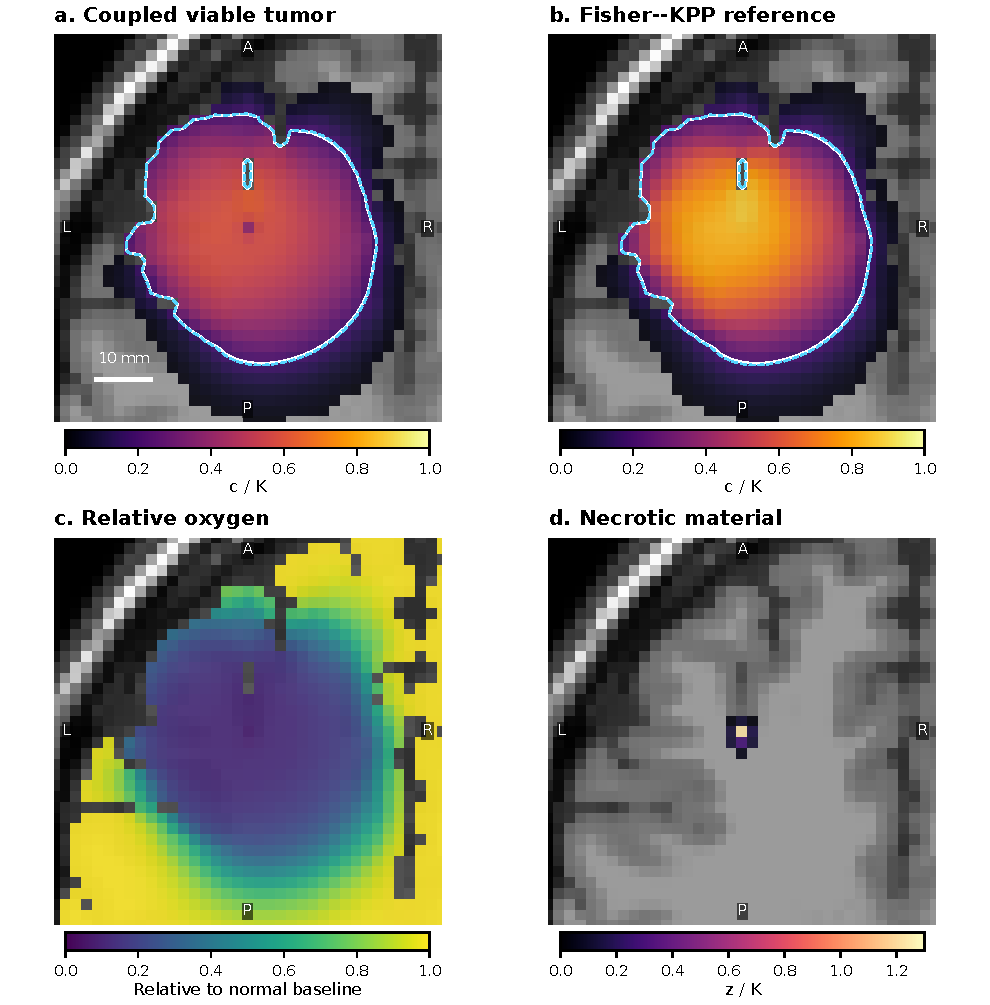
\includegraphics[width=0.94\textwidth]{figures/day90_fields.pdf}
\caption{Day-90 fields in the matched primary simulations. Axial views at RAS $z=30$ mm show a $72\times72$ mm region, with the original 2 mm simulation pixels retained. Viable density and the reference share the same $0$--$1$ color scale; oxygen is relative to the normal baseline. Necrotic material is shown over $0$--$1.3$ without clipping its peak at one. White solid and cyan dashed contours mark $c/K=0.2$ in M2 and M0, respectively. Tumor/necrosis overlays below 0.02 of $K$ are transparent for display only. The scale bar is 10 mm. These thresholds and colors have no calibrated correspondence to MRI contrast.}\label{fig:fields}
\end{figure}

Minimum tissue oxygen in M2 was \MinimumOxygen{}. Necrotic material totaled \NecroticCells{} million cell equivalents, with $z/K\geq0.2$ occupying \NecroticVolume{} mL, or three 2 mm voxels. Low-oxygen volume ($o<0.1$) was 0.104 mL. The dense initial seed was already oxygen limited; this experiment therefore does not demonstrate the spontaneous emergence of a macroscopic necrotic core from a dilute initial tumor. The tiny thresholded focus is not a resolved anatomical cavity. Moreover, the maximum $z/K=\MaximumNecrosis{}$ exceeds one, as permitted by the cell-equivalent formulation.

The viable-count gap between M0 and M2 was \CellGapMillion{} million cells. Only \NecroticCells{} million cell equivalents were stored as necrotic material. With no clearance, the remaining \BirthGapMillion{} million difference in live-plus-dead burden is attributable to reduced cumulative births in the discrete balance. Thus, in this case, the smaller viable burden mainly reflects inhibited proliferation rather than death transfer.

\subsection{Controlled model ablations}
Table~\ref{tab:ablations} and Figure~\ref{fig:curves} separate growth inhibition, death transfer and the chosen supply feedback. Removing hypoxic death (M1) increased day-90 viable count by approximately 0.14\% relative to M2. In contrast, removing burden-dependent suppression of oxygen supply ($\alpha=0$) gave 2.829 billion viable cells, approximately 0.62\% below M0. Its minimum oxygen, 0.2245, remained above the death threshold, and no necrotic material formed. The supply closure therefore has a much larger effect on this particular comparison than the death term. This finding is conditional on the assigned parameters and dense seed, and does not establish the closure biologically.

\begin{table}[tbp]
\centering\small
\caption{Day-90 outcomes for 2 mm model ablations with a maximum 0.25-day step. $V_{0.2}$ and $V_{0.8}$ are viable-density threshold volumes in mL. Oxygen and necrotic state variables are absent from M0, indicated by dashes.}\label{tab:ablations}
\setlength{\tabcolsep}{4pt}
\begin{tabularx}{\textwidth}{Yrrrrr}
\toprule Model & $N_c/10^9$ & $V_{0.2}$ & $V_{0.8}$ & $\min o$ & $N_z/10^6$\\\midrule
\AblationRows
\bottomrule
\end{tabularx}
\end{table}

Setting uptake to zero ($\beta=0$) maintained $o=1$, yielded no necrotic material and reproduced the M0 solution. The largest final density discrepancy divided by $K$ was below $10^{-5}$, consistent with finite-precision differences between the numerical paths. This is a limiting-case verification, not an independent biological comparison.

\begin{figure}[p]
\centering
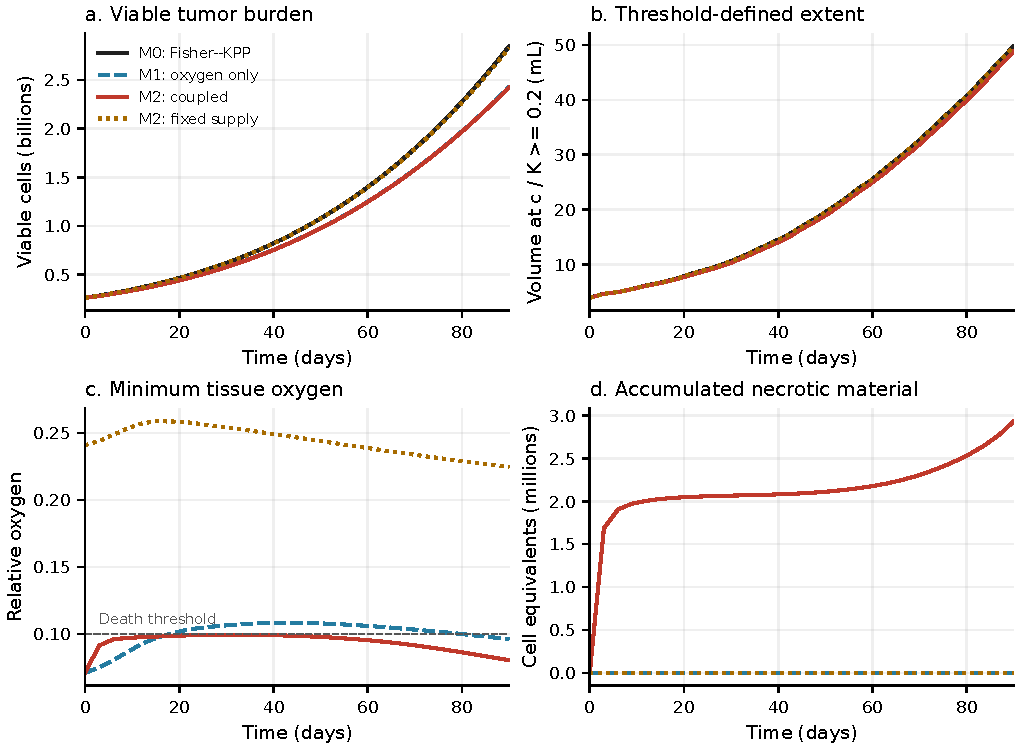
\includegraphics[width=\textwidth]{figures/timecourses.pdf}
\caption{Time courses for the matched reference and selected ablations. Panels show viable cell count, threshold-defined viable volume, minimum tissue oxygen and necrotic cell equivalents. M0 has no oxygen or necrosis state; these curves are consequently omitted. The dashed horizontal line in panel c marks $\theta_d=0.1$. M1 and M2 burden curves nearly overlap. All curves are deterministic simulations with assigned parameters; they are not measurements, replicate averages or uncertainty intervals.}\label{fig:curves}
\end{figure}

\subsection{Numerical verification and resolution dependence}
The software test suite passed all \TestCount{} tests. Checks include analytical logistic behavior, diffusion conservation, boundary behavior, positivity, death-transfer balance, oxygen bounds and model limits (Appendix~\ref{app:numerics}). These results verify implemented properties without validating the biological assumptions.

At 2 mm, reducing the maximum time step from 0.25 to 0.125 day decreased the final relative $L^2$ difference in viable density against the 0.0625-day calculation from 0.1270\% to 0.0423\%. Corresponding necrotic-field differences decreased from 4.238\% to 1.386\%. The relative oxygen differences were 0.0129\% and 0.0043\%. These comparisons support temporal refinement of the implemented scheme; a finite reference calculation does not provide an exact error or establish an asymptotic convergence order.

\begin{table}[tbp]
\centering\small
\caption{Day-90 outcomes under temporal and anatomical-grid refinement for M2. $h$ is voxel spacing in mm and $\Delta t$ is the maximum step in days. The 1 mm run changes both the numerical mesh and the discretized tissue boundaries.}\label{tab:refinement}
\begin{tabular}{rrrrrr}
\toprule $h$ & $\Delta t$ & $N_c/10^9$ & $N_z/10^6$ & $\min o$ & $\max(z/K)$\\\midrule
\RefinementRows
\bottomrule
\end{tabular}
\end{table}

The native 1 mm calculation contained 2.452 billion viable cells, compared with 2.878 billion in its matched M0 reference, a \NativeCellReduction\% reduction. This relative reduction is similar to the primary result. However, minimum oxygen fell to \NativeMinimumOxygen{}, the necrotic-equivalent count increased to 3.607 million and peak $z/K$ rose to \NativeMaximumNecrosis{}. The necrotic threshold occupied 0.032 mL (32 native voxels), while low-oxygen volume was 0.027 mL. These local quantities are sensitive to spatial resolution and to the discrete anatomy. Neither grid resolves the assigned 0.2 mm oxygen length; spatial convergence of the oxygen--necrosis subsystem has not been demonstrated.

\subsection{Homogeneous parameter recovery and uncertainty}\label{sec:recovery_results}
In the separate homogeneous experiment, all three initial guesses converged to the same fit at the reported precision. Estimated diffusion was \RecoveryDEstimate{} mm$^2$/day and proliferation was \RecoveryRhoEstimate{} day$^{-1}$, relative errors of \RecoveryDRelativeError\% and \RecoveryRhoRelativeError\%, respectively (Table~\ref{tab:recovery}). Both known values lay within the local and bootstrap marginal 95\% intervals. The log-parameter correlation was \RecoveryCorrelation{}, indicating that uncertainty in the two rates should be propagated jointly. No primary or replicate fit reached a bound or failed. Agreement across starts and finite sensitivity singular values support local estimation for this experiment; they do not establish global identifiability under unknown initialization.

\begin{table}[tbp]
\centering\small
\caption{Recovery from the first three noisy scans of the homogeneous phantom. Local intervals use the known-noise residual Jacobian; bootstrap intervals are percentiles of \RecoveryBootstraps{} refits. Intervals are marginal, frequentist and conditional on known initialization and imaging assumptions.}\label{tab:recovery}
\setlength{\tabcolsep}{4pt}
\begin{tabularx}{\textwidth}{lrrYY}
\toprule Parameter & Known & Estimate & Local 95\% CI & Bootstrap 95\% CI\\\midrule
\RecoveryRows
\bottomrule
\end{tabularx}
\end{table}

Across \RecoveryTrials{} independent noise realizations, local intervals covered $D$ in \RecoveryDCoverageCount/\RecoveryTrials{} trials and $\rho$ in \RecoveryRhoCoverageCount/\RecoveryTrials{} trials (Table~\ref{tab:recovery_coverage}; Figure~\ref{fig:recovery}). The exact binomial intervals include the nominal 95\% rate and remain broad. The observed 98.3\% and 100\% fractions therefore neither establish exact calibration nor imply guaranteed coverage. The study varies measurement noise at one fixed biology, initialization and imaging setting, rather than sampling a virtual patient population. The time-zero-only control was correctly rejected as locally unidentifiable.

\begin{table}[tbp]
\centering\small
\caption{Independent repeated-noise recovery audit of local 95\% intervals. Bias and RMSE retain the units in the parameter column. The last column quantifies sampling uncertainty in empirical coverage, not uncertainty in an individual parameter estimate.}\label{tab:recovery_coverage}
\setlength{\tabcolsep}{4pt}
\begin{tabularx}{\textwidth}{lrrYY}
\toprule Parameter & Bias & RMSE & Coverage & Binomial 95\% CI\\\midrule
\RecoveryCoverageRows
\bottomrule
\end{tabularx}
\end{table}

\begin{figure}[p]
\centering
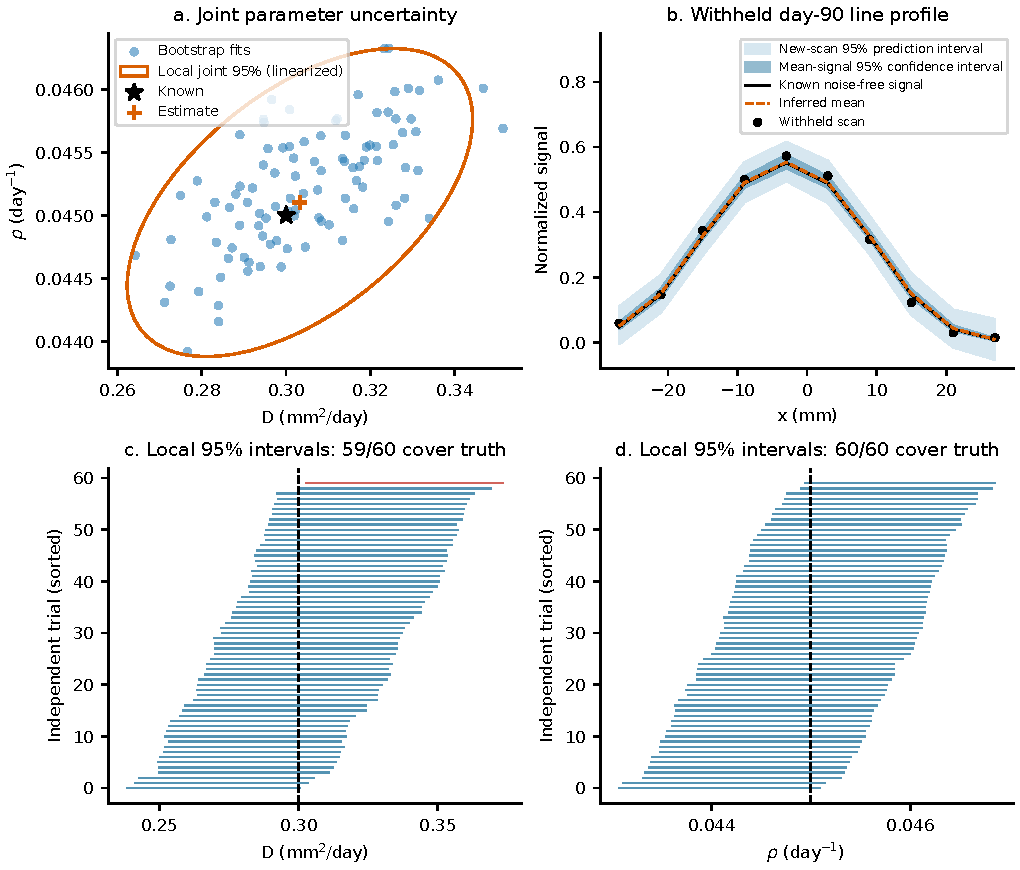
\includegraphics[width=\textwidth]{figures/synthetic_recovery.pdf}
\caption{Synthetic recovery and conditional uncertainty. (a) Joint bootstrap estimates and a local joint 95\% ellipse, linearized into physical units. The star marks the known rates. (b) A day-90 line profile through the nearest observation-voxel centers to the seed's $y,z$ coordinates. The darker mean-signal confidence band accounts for parameter uncertainty; the lighter new-scan prediction band also includes independent noise. Both are pointwise intervals. (c,d) Local marginal 95\% intervals for the \RecoveryTrials{} independent noise realizations, sorted by fitted rate. Red denotes a missed known value; the dashed line is ground truth. These trials audit local intervals, not bootstrap coverage or clinical variability.}\label{fig:recovery}
\end{figure}

\subsection{Withheld homogeneous forecasts and numerical discrepancy}
Day-75 and day-90 predictions used no observations beyond day 60. Whole-image RMSE against the known noise-free signal was $4.72\times10^{-4}$ and \RecoveryDayNinetyRMSE{}, respectively, while RMSE against the withheld noisy images was approximately the 0.03 noise standard deviation (Table~\ref{tab:recovery_forecast}). The 95\% new-scan prediction intervals contained 94.0\% and 94.6\% of the withheld voxel measurements. These are spatial fractions in two scans, not coverage estimates from independent patients; the whole-box metrics include background voxels. Figure~\ref{fig:recovery}b separately displays the signal near the tumor. Confidence in the mean signal is narrower than prediction uncertainty for a future noisy measurement.

\begin{table}[tbp]
\centering\small
\caption{Withheld synthetic-scan forecast errors in normalized signal units, evaluated over all 1,000 observation voxels per scan. Prediction intervals are approximate and pointwise, conditional on the fitted model.}\label{tab:recovery_forecast}
\begin{tabularx}{\textwidth}{rYYY}
\toprule Day & RMSE vs clean truth & RMSE vs noisy scan & Voxel fraction in 95\% prediction interval\\\midrule
\RecoveryForecastRows
\bottomrule
\end{tabularx}
\end{table}

At day 90, the observation-space RMSE between the inference grid and fine generator at the known parameters was \RecoveryDayNinetyGridRMSE{}, approximately 1.14\% of the noise standard deviation. Halving the inference time step changed the signal by RMSE \RecoveryDayNinetyTimeRMSE{}. The finer generator is still a numerical reference, and a small per-voxel discrepancy does not by itself ensure negligible bias when many voxels are used; the repeated-noise audit supplies a complementary check.


\subsection{BrainWeb tissue-specific parameter recovery}\label{sec:bw_results}
The three starting guesses agreed to the reported precision. The estimated $(D_{\rm WM},D_{\rm GM},\rho)$ was $(\BWWhiteEstimate,\BWGrayEstimate,\BWRhoEstimate)$, with relative errors \BWWhiteError\%, \BWGrayError\% and \BWRhoError\%, respectively (Table~\ref{tab:bw_recovery}). Both diffusion truths lay within the local and bootstrap 95\% intervals. The true $\rho=0.040$ day$^{-1}$ fell just above their respective upper limits, 0.039968 and 0.039920 day$^{-1}$. This noise realization and its interval misses were retained. No primary, bootstrap or independent-trial fit failed or reached a bound.

\begin{table}[tbp]
\centering\small
\caption{Three-rate recovery from noisy BrainWeb signals. Units are mm$^2$/day for diffusion and day$^{-1}$ for proliferation. Intervals are marginal and conditional on the known seed, anatomy, imaging model and noise. The true proliferation rate is outside both intervals in this realization.}\label{tab:bw_recovery}
\setlength{\tabcolsep}{3pt}
\begin{tabularx}{\textwidth}{lrrYY}
\toprule Parameter & Known & Estimate & Local 95\% CI & Bootstrap 95\% CI\\\midrule
\BWRecoveryRows
\bottomrule
\end{tabularx}
\end{table}

Gray-matter diffusion had the widest relative uncertainty. The log-rate correlation between white- and gray-matter diffusion was \BWCorrelation{} (Figure~\ref{fig:bw_recovery}a). Weighted sensitivity singular values were approximately 184.35, 24.64 and 5.25, with Jacobian condition number \BWCondition{}. These local diagnostics support estimating three rates for this specific design, without proving global identifiability or robustness to uncertain initialization. Time-zero-only data were correctly rejected. A separate unit test rejected two-tissue inference in an all-white-matter domain.

Across \BWTrials{} independent noise datasets, local 95\% interval coverage was \BWWhiteCoverage/\BWTrials{} for $D_{\rm WM}$, \BWGrayCoverage/\BWTrials{} for $D_{\rm GM}$ and \BWRhoCoverage/\BWTrials{} for $\rho$ (Table~\ref{tab:bw_coverage}; Figure~\ref{fig:bw_recovery}d--f). Exact binomial intervals include 95\% but are broad. Repeated-noise biases were small relative to single-fit uncertainty; the audit neither guarantees nominal coverage nor evaluates bootstrap coverage. The primary proliferation miss is compatible with sampling variation rather than grounds for replacing the noise seed.

\begin{table}[tbp]
\centering\small
\caption{BrainWeb repeated-noise audit of local 95\% intervals. Bias and RMSE retain the units shown. Binomial intervals describe Monte Carlo uncertainty in the coverage fraction, not uncertainty in a fitted rate.}\label{tab:bw_coverage}
\setlength{\tabcolsep}{3pt}
\begin{tabularx}{\textwidth}{lrrYY}
\toprule Parameter & Bias & RMSE & Coverage & Binomial 95\% CI\\\midrule
\BWCoverageRows
\bottomrule
\end{tabularx}
\end{table}

\begin{figure}[p]
\centering
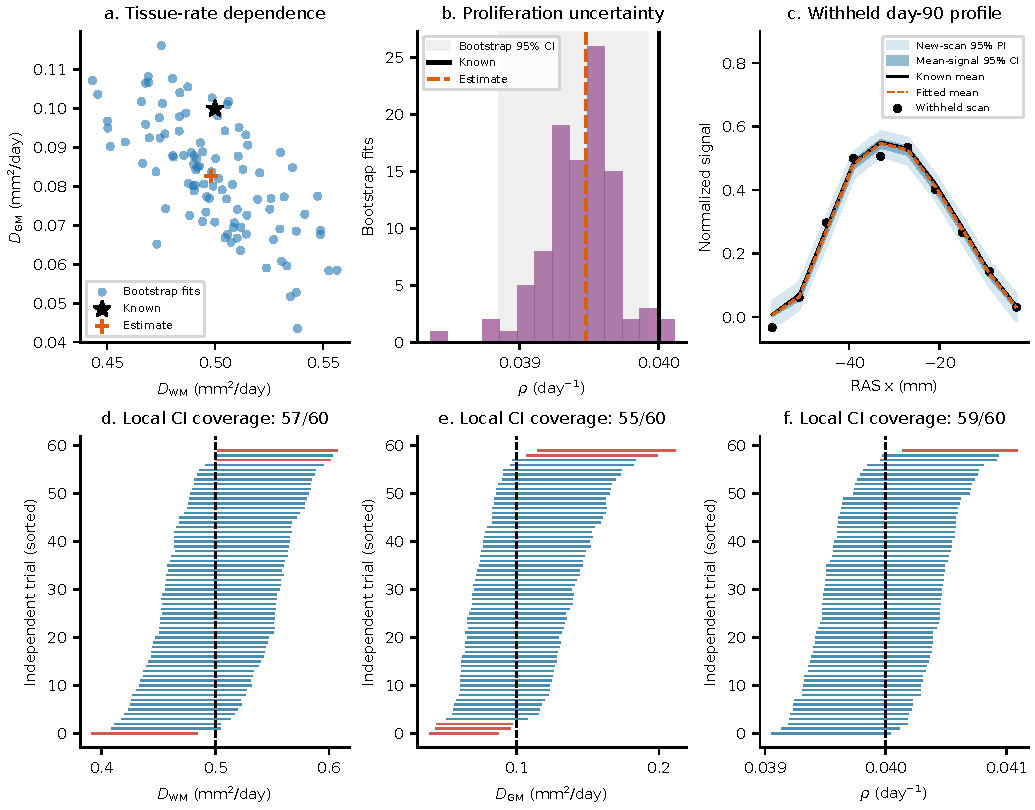
\includegraphics[width=\textwidth]{figures/brainweb_recovery.pdf}
\caption{BrainWeb recovery and conditional uncertainty. (a) Joint white-/gray-matter bootstrap estimates; the star denotes known rates and the cross the primary estimate. (b) Proliferation bootstrap distribution, with marginal percentile interval shading; its known value is just beyond the upper limit. (c) Withheld day-90 profile through the nearest observation-voxel centers to the seed's $y,z$ coordinates. Mean-signal confidence and new-scan prediction intervals are pointwise and have different meanings. (d--f) Local 95\% intervals for 60 independent noise realizations, sorted by fitted rate. Red marks a missed known value. These repetitions share anatomy and biology and do not constitute a virtual patient cohort.}\label{fig:bw_recovery}
\end{figure}

\subsection{BrainWeb withheld forecasts and anatomy sensitivity}\label{sec:bw_sensitivity}
Day-90 RMSE against the noise-free signal was \BWDayNinetyRMSE{} over the full FOV and \BWNearDayNinetyRMSE{} in the prespecified near-seed region (Table~\ref{tab:bw_forecast}). New-scan prediction intervals contained 94.2\% of all withheld day-90 voxels but only 89.2\% of near-seed voxels. Thus, background-inclusive summaries can conceal less favorable performance near the tumor. These are descriptive spatial fractions for one noisy scan, not independent coverage trials or simultaneous spatial guarantees.

\begin{table}[tbp]
\centering\small
\caption{Withheld BrainWeb forecast metrics. The full FOV contains 1,000 observation voxels; the near-seed region contains 120. Errors use normalized signal units. The final column is the spatial fraction of noisy observations in approximate pointwise 95\% new-scan prediction intervals.}\label{tab:bw_forecast}
\begin{tabularx}{\textwidth}{rlYYY}
\toprule Day & Region & RMSE vs clean & RMSE vs noisy & Voxel fraction in prediction interval\\\midrule
\BWForecastRows
\bottomrule
\end{tabularx}
\end{table}

On the shared 3 mm anatomy, changing the maximum step from 0.5 to 0.25 day reduced day-90 signal RMSE relative to the 0.125-day generator from \BWDayNinetyTimeRMSE{} to \BWHalfTimeRMSE{}. By contrast, the 3 mm versus 2 mm generator discrepancy at the known rates reached \BWDayNinetyGridRMSE{} at day 90, or 18.4\% of the 0.02 noise standard deviation (Figure~\ref{fig:bw_anatomy}). This is a change in discretized anatomy and numerical representation rather than a pure spatial-convergence comparison.

Fitting the noise-free 2 mm signal with the 3 mm model estimated $D_{\rm GM}=\BWGrayStressEstimate$ mm$^2$/day, a +\BWGrayStressShift\% shift from the known value (Table~\ref{tab:bw_anatomy}). Corresponding white-matter and proliferation shifts were +0.04\% and -0.13\%. The paired noisy stress fit gave $(0.499160,0.096770,0.039445)$ in the respective units. Its conditional local intervals do not incorporate anatomy/grid discrepancy. Signal error below one noise standard deviation per voxel can therefore coexist with a material rate shift when systematic differences are fitted across many measurements. This sensitivity example does not estimate segmentation uncertainty or establish a universal gray-matter bias.

\begin{table}[tbp]
\centering\small
\caption{Anatomy/grid sensitivity: full 2 mm data fitted with the 3 mm model. The noiseless fit isolates a deterministic rate shift under the changed representation. The noisy fit reuses the primary observation-noise draw. Neither fit estimates a distribution of anatomy uncertainty.}\label{tab:bw_anatomy}
\setlength{\tabcolsep}{3pt}
\begin{tabularx}{\textwidth}{lrrrY}
\toprule Parameter & Known & Noiseless fit & Relative shift & Paired noisy fit\\\midrule
\BWAnatomyRows
\bottomrule
\end{tabularx}
\end{table}

\begin{figure}[p]
\centering
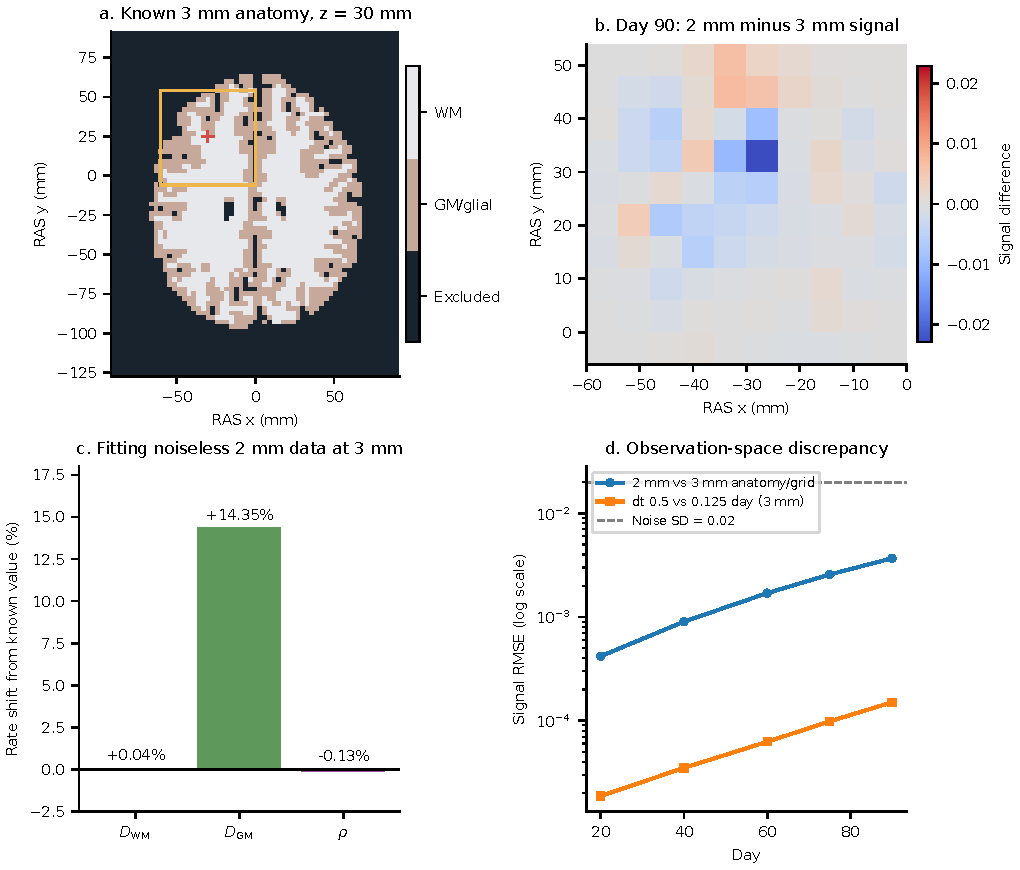
\includegraphics[width=\textwidth]{figures/brainweb_anatomy_sensitivity.pdf}
\caption{Sensitivity to anatomy and numerical representation. (a) Full 3 mm tissue domain at RAS $z=30$ mm, with the known seed center and fixed 60 mm observation FOV. The forward PDE is not cropped to that box. (b) Difference between 2 mm and 3 mm noise-free generating signals at day 90, using identical physical observation voxels; the displayed observation plane is at $z=27$ mm. (c) Relative shifts after fitting the noise-free 2 mm data with the 3 mm inverse model. (d) Observation-space discrepancies at the known rates; temporal error on the shared 3 mm grid is smaller than the combined anatomy/grid effect. Both generators in the anatomy comparison use a 0.125-day step. No biological measurement or clinical validation is represented.}\label{fig:bw_anatomy}
\end{figure}

The two phantom recovery experiments fit synthetic M0 observations only; the subsequent PAT16 recovery uses its tensor-transport counterpart. The oxygen--necrosis parameters and the dense-seed forward comparisons remain assigned inputs; no patient parameters, oxygen/death rates or clinical predictive errors were estimated.
\FloatBarrier

\subsection{PAT16 conditional MRI-informed comparison}\label{sec:pat16_results}
The shared grid contained $51\times62\times50$ voxels, with 44,667 active tissue voxels and 18,202 eligible directional white-matter voxels. A lesion override included 603 voxels classified as CSF by the healthy-tissue segmentation, using assumed gray-matter transport. Resampled tensor-derived FA correlated with the saved T1-space FA at $r=\PATFAR$; this is transformation consistency, not independent registration validation. Of 180 BOLD frames, 157 remained after censoring. The nuisance design had rank 36, leaving 121 algebraic residual degrees of freedom. These counts do not correct for temporal autocorrelation or quantify FC reliability.

Day-90 marginal median normalized burden was 110.42 mL equivalents for isotropic and 106.74 for anisotropic transport (Table~\ref{tab:pat16_outcomes}). The paired median difference was $\PATBurdenDifference$ mL equivalents, with 5th--95th percentiles $[-6.80,-0.85]$. For the illustrative $u\geq0.16$ volume, the paired difference was $-6.36$ mL, with percentiles $[-12.83,-2.46]$. A paired-difference median is computed scenario by scenario and need not equal the difference of the two marginal medians. These are simulated, parameter-dependent effects, not observed changes in the patient.

\begin{table}[tbp]
\centering\small
\caption{PAT16 day-90 conditional outcomes: median [5th, 95th percentile] across \PATScenarios{} paired assumed-parameter scenarios. Differences are anisotropic minus isotropic. The bands are empirical sensitivity ranges, not calibrated patient intervals; the density threshold has no validated MRI correspondence.}\label{tab:pat16_outcomes}
\setlength{\tabcolsep}{3pt}
\begin{tabularx}{\textwidth}{Y Y Y Y}
\toprule Quantity & Isotropic & Anisotropic & Paired difference\\\midrule
\PATRows
\bottomrule
\end{tabularx}
\end{table}

\begin{figure}[p]
\centering
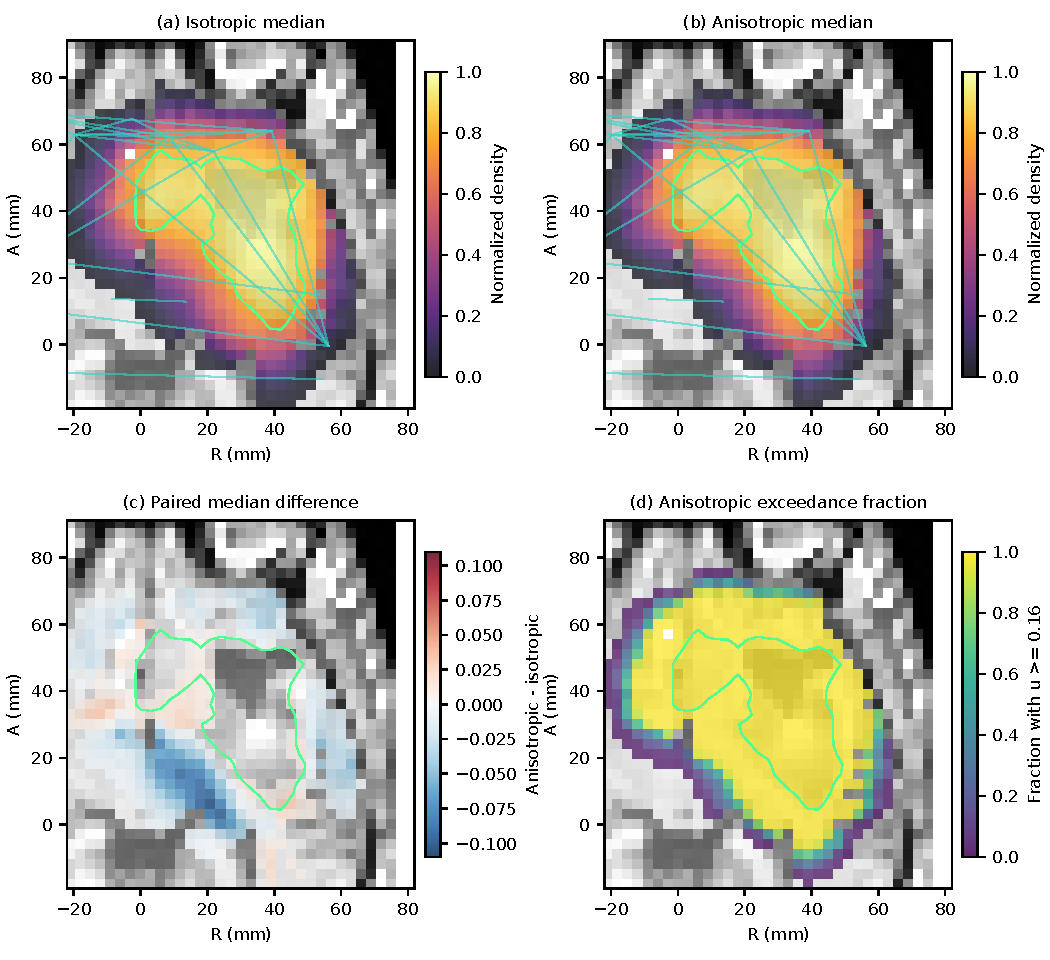
\includegraphics[width=\textwidth]{figures/pat16_fields.pdf}
\caption{PAT16 conditional day-90 growth on the preoperative axial plane at RAS $z=-12$ mm. (a,b) Pointwise marginal median normalized density with shared colors. (c) Median of paired anisotropic-minus-isotropic fields, with the full displayed difference range retained. (d) Fraction of assumed scenarios exceeding $u=0.16$, not a calibrated probability of tumor presence. Green contours show the input lesion at threshold 0.5. Cyan/purple lines in (a,b) are measured positive/negative FC projected from ROI centers within a $\pm12$ mm slab, not anatomical tracts on the slice. Background T1, lesion and FC are measurement-derived; growth is simulated. No functional decline is predicted. Values below 0.02 (absolute difference below 0.005 in panel c) are transparent for display only.}\label{fig:pat16_fields}
\end{figure}

The spatial comparison shows redistribution associated with directional transport (Figure~\ref{fig:pat16_fields}). Marginal global bands substantially overlapped throughout the run (Figure~\ref{fig:pat16_curves}). Regional mean-density summaries and measured static connectivity are supplied with the notebook; they do not constitute network or cognitive forecasts. No later patient scan was used to evaluate the hypothetical untreated evolution.

All paired initial states matched, and recorded densities remained between zero and 0.99733 without clipping. Every scenario used a 0.5-day step. For a representative central anisotropic scenario, halving the step changed day-90 density by \PATTimeDifference\% in relative $L^1$. A five-day pure-diffusion test gave relative mass error $5.69\times10^{-10}$ after float32 output storage. Additional tests verify tensor reconstruction and mixed derivatives, isotropic equivalence, a rotated Gaussian's covariance growth, coordinate transforms, conservation and blocked-corner behavior. These checks support implementation correctness and limited temporal sensitivity; spatial convergence on the PAT16 tissue graph and independent patient prediction have not been demonstrated.

\begin{figure}[tbp]
\centering
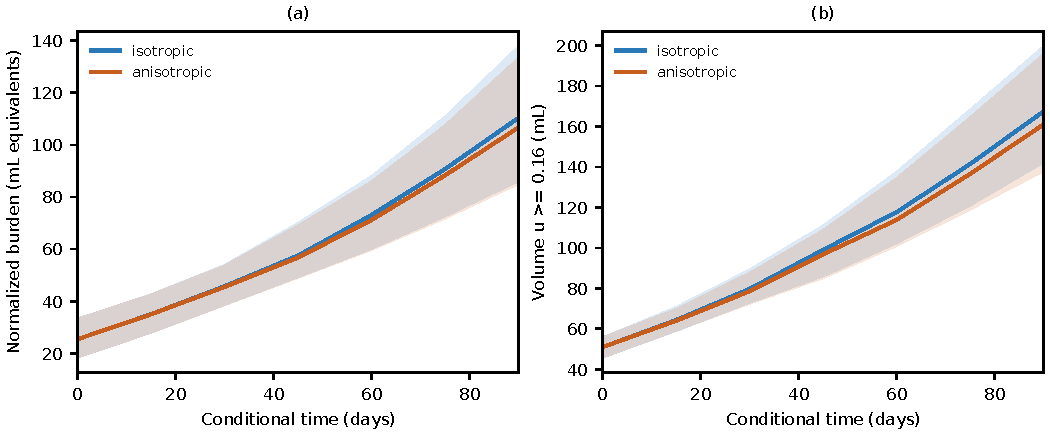
\includegraphics[width=\textwidth]{figures/pat16_timecourses.pdf}
\caption{PAT16 simulated normalized burden and illustrative threshold-defined volume. Lines are marginal medians and shading denotes 5th--95th empirical percentiles over the same \PATScenarios{} paired assumed scenarios. Time zero is lesion-based initialization, not tumor onset. No surgery, radiation, drug effect or oxygen limitation is included. Wide overlapping marginal bands coexist with the negative paired differences in Table~\ref{tab:pat16_outcomes}.}\label{fig:pat16_curves}
\end{figure}
\FloatBarrier

\subsection{PAT16 four-parameter recovery and conditional uncertainty}\label{sec:pat16_recovery_results}
The three starts converged to practically identical estimates. The fitted $(D_{\rm WM},D_{\rm GM},\rho,r)$ was $(\PRWhiteEstimate,\PRGrayEstimate,\PRRhoEstimate,\PRRatioEstimate)$ (Table~\ref{tab:pat16_recovery}). Relative errors were $\PRWhiteError\%$, $\PRGrayError\%$, $\PRRhoError\%$ and $\PRRatioError\%$, respectively. All four generating values lay inside both local and bootstrap marginal 95\% intervals. This does not imply joint 95\% coverage of the four-dimensional parameter vector. No primary, bootstrap or independent-noise fit failed or reached a search bound. These results concern generated signals on patient-derived anatomy; they do not recover biological rates from PAT16 measurements.

\begin{table}[tbp]
\centering\small
\caption{Synthetic four-parameter recovery on PAT16 anatomy. Marginal intervals condition on fixed anatomy, dMRI directions, normalized initialization and signal/noise calibration. They do not estimate absolute capacity. The original pilot's sensitivity percentiles are a separate uncertainty construction.}\label{tab:pat16_recovery}
\setlength{\tabcolsep}{3pt}
\begin{tabularx}{\textwidth}{lrrYY}
\toprule Parameter & Known & Estimate & Local 95\% CI & Bootstrap 95\% CI\\\midrule
\PRRecoveryRows
\bottomrule
\end{tabularx}
\end{table}

WM diffusivity and anisotropy were positively dependent, with local log-parameter correlation \PRWMRatioCorrelation{} (Figure~\ref{fig:pat16_recovery}b,c). Weighted Jacobian singular values were approximately \PRSingularValues{}, with condition number \PRCondition{}. Training standardized residual RMS was \PRTrainingRMS{}. These diagnostics support local estimation under this initialization and observation design, without establishing global identifiability or robustness to unknown directions and initial density.

\begin{figure}[p]
\centering
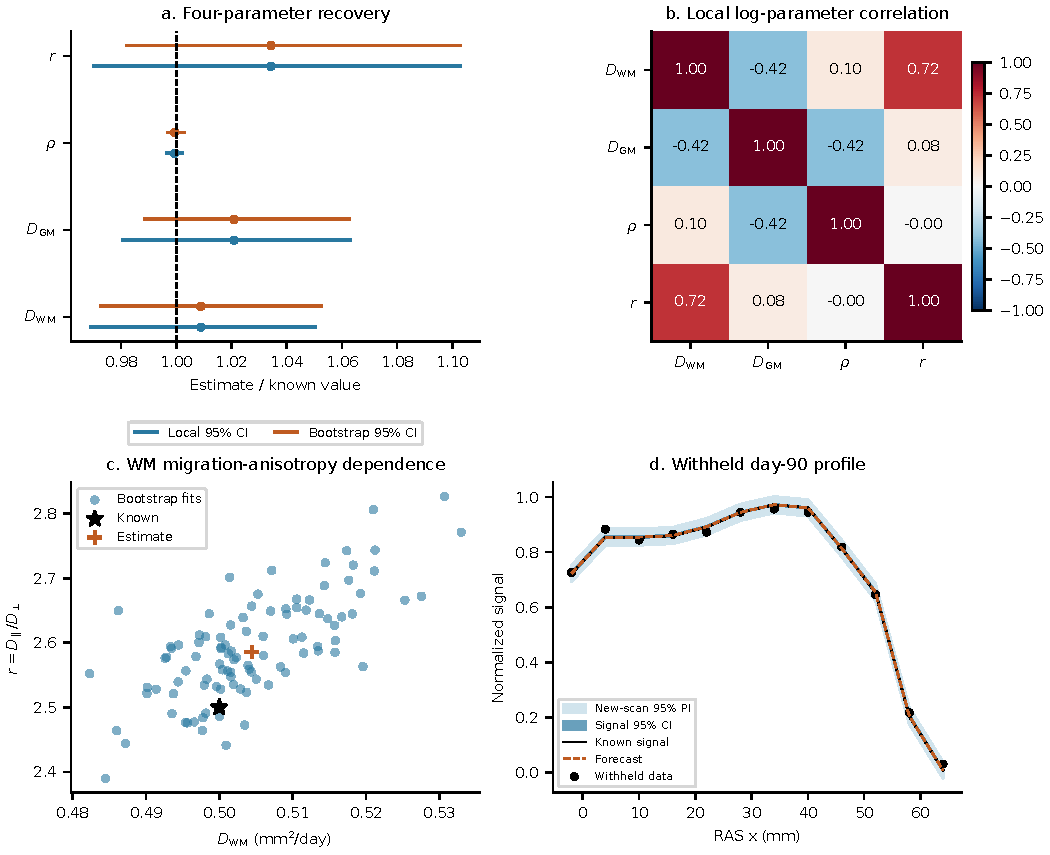
\includegraphics[width=\textwidth]{figures/pat16_recovery.pdf}
\caption{PAT16 synthetic recovery and uncertainty. (a) Primary estimates divided by the known generating values, with local and bootstrap marginal 95\% confidence intervals; the dashed line denotes truth. (b) Local log-parameter correlations. (c) All \PRBootstraps{} bootstrap WM-diffusivity/anisotropy pairs, with known values and the primary estimate. (d) A fixed central observation-voxel row at withheld day 90, showing nominal pointwise 95\% signal confidence and Gaussian-mixture new-measurement prediction intervals. The observation row uses $y=\PRProfileY$, $z=\PRProfileZ$ mm in RAS coordinates. No later measurement enters fitting or resampling. The joint dependence should be propagated; separate marginal endpoints do not define independent parameter combinations.}\label{fig:pat16_recovery}
\end{figure}

Across \PRTrials{} independent noise datasets, marginal local-interval coverage was \PRWhiteCoverage/\PRTrials{}, \PRGrayCoverage/\PRTrials{}, \PRRhoCoverage/\PRTrials{} and \PRRatioCoverage/\PRTrials{} (Table~\ref{tab:pat16_recovery_coverage}; Figure~\ref{fig:pat16_recovery_validation}). Mean relative biases were $\PRWhiteBias\%$, $\PRGrayBias\%$, $\PRRhoBias\%$ and $\PRRatioBias\%$. Exact binomial intervals contained the nominal 95\% level but remained broad; this is not evidence of established 95\% calibration. The audit includes the declared temporal mismatch while holding anatomy, directions, initialization and observation calibration fixed. It does not assess marginal bootstrap parameter-interval coverage or robustness to broader model error.

\begin{table}[tbp]
\centering\small
\caption{PAT16 independent-noise audit of local 95\% intervals. Bias is relative to the known parameter; RMSE uses the parameter's units. Exact binomial intervals quantify Monte Carlo uncertainty in coverage. Failed/boundary intervals would count as misses; none occurred.}\label{tab:pat16_recovery_coverage}
\setlength{\tabcolsep}{3pt}
\begin{tabularx}{\textwidth}{lrrYY}
\toprule Parameter & Mean bias & RMSE & Local coverage & Exact 95\% binomial CI\\\midrule
\PRCoverageRows
\bottomrule
\end{tabularx}
\end{table}

\begin{figure}[p]
\centering
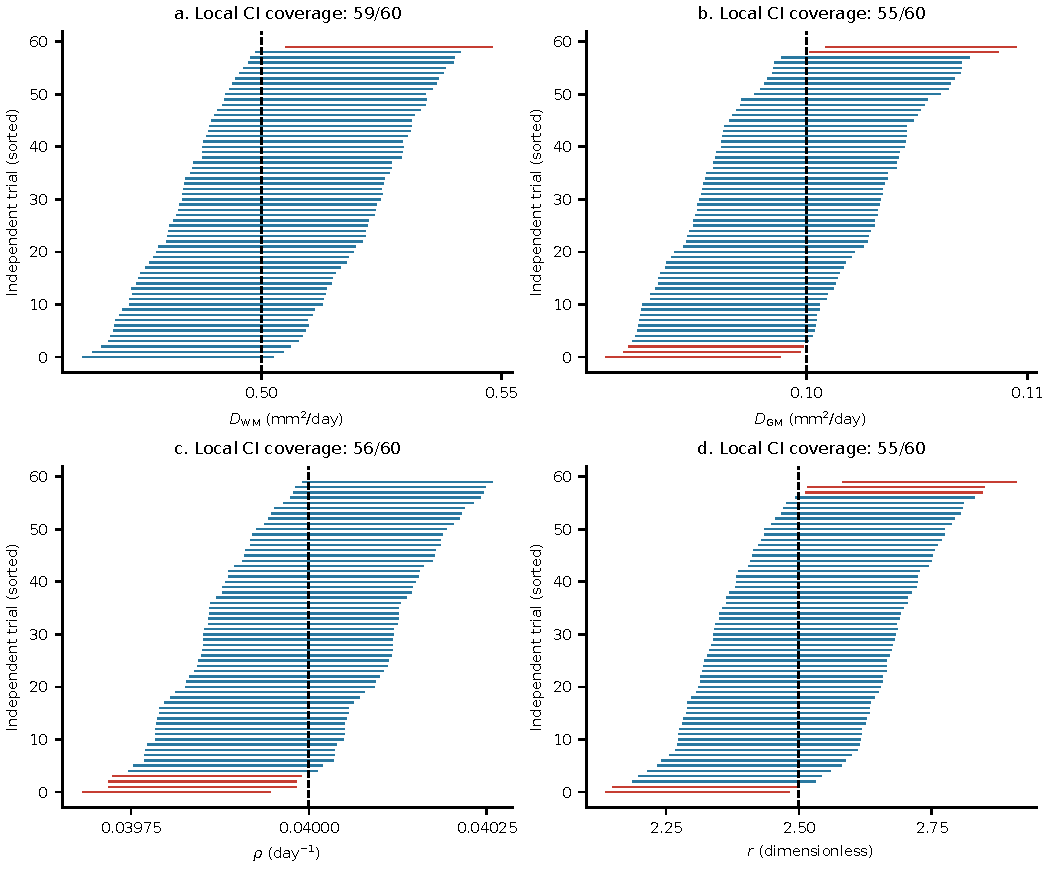
\includegraphics[width=\textwidth]{figures/pat16_recovery_validation.pdf}
\caption{Validation against known synthetic generating parameters on PAT16 anatomy across \PRTrials{} fresh noise datasets. Each segment is a marginal local 95\% interval, sorted within parameter by fitted value; the black dashed line is the known value. Red intervals miss truth. Counts include all attempted trials. These repetitions share anatomy, initialization, directions, biology and observation calibration; they are independent noise realizations, not independent patients. Exact binomial intervals and parameter bias/RMSE are reported in Table~\ref{tab:pat16_recovery_coverage}.}\label{fig:pat16_recovery_validation}
\end{figure}

\subsection{PAT16 withheld forecasts and numerical validation}\label{sec:pat16_recovery_forecast}
Full-cube forecast RMSE against the noise-free signal was \PRDaySeventyFiveRMSE{} at day 75 and \PRDayNinetyRMSE{} at day 90, while noisy-scan RMSE was approximately the assumed 0.015 noise standard deviation (Table~\ref{tab:pat16_recovery_forecast}). The nominal pointwise 95\% signal intervals contained \PRDaySeventyFiveSignalContainment\% and \PRDayNinetySignalContainment\% of full-cube truth values. Final Gaussian-mixture prediction intervals contained \PRDaySeventyFivePredictionContainment\% and \PRDayNinetyPredictionContainment\% of noisy observations; near-center fractions were \PRNearDaySeventyFivePredictionContainment\% and \PRNearDayNinetyPredictionContainment\%. These descriptive spatial fractions do not establish repeated or simultaneous coverage.

Mean full-cube signal-interval widths were \PRDaySeventyFiveSignalWidth{} and \PRDayNinetySignalWidth{}; final prediction widths were \PRDaySeventyFivePredictionWidth{} and \PRDayNinetyPredictionWidth{} normalized signal units at days 75/90. The original 100 noisy draws gave about 93.2\%/93.1\% containment and widths 0.05642/0.05639. Increasing predictive draws to 1,000 and \PPDraws{} reduced interval-endpoint RMSE against the integrated mixture from \PPEndpointLegacy{} to \PPEndpointThousand{} and \PPEndpointMany{}, respectively (Figure~\ref{fig:pat16_prediction_validation}a). Integration removes noise-tail sampling error without tuning widths; the number of distinct parameter vectors remains \PRBootstraps{}.

\begin{table}[tbp]
\centering\small
\caption{Withheld PAT16 forecast validation. The full FOV contains 1,728 observation voxels and the near-center sphere 280. Signal RMSE is against noise-free truth. The noisy RMSE is divided by the known noise SD. The last two columns report spatial containment in nominal pointwise 95\% signal confidence and Gaussian-mixture new-observation prediction intervals, respectively. These fractions are not an independent coverage audit.}\label{tab:pat16_recovery_forecast}
\setlength{\tabcolsep}{3pt}
\begin{tabularx}{\textwidth}{rlYYYY}
\toprule Day & Region & Signal RMSE & Noisy RMSE/SD & Truth in signal CI & Data in prediction interval\\\midrule
\PRForecastRows
\bottomrule
\end{tabularx}
\end{table}

Across \PPTrials{} independently regenerated datasets and \PPNestedFits{} nested bootstrap refits, full-cube mean coverage was \PPOldFullSeventyFive\%/\PPOldFullNinety\% for 100 noisy draws, \PPManyFullSeventyFive\%/\PPManyFullNinety\% for \PPDraws{} draws and \PPMixFullSeventyFive\%/\PPMixFullNinety\% for integrated intervals at days 75/90 (Table~\ref{tab:pat16_prediction_validation}). The integrated mean-coverage Monte Carlo 95\% intervals were \PPMixFullSeventyFiveCI\% and \PPMixFullNinetyCI\%; near-center mean coverage was \PPMixNearSeventyFive\% and \PPMixNearNinety\%. Day-75 full-cube coverage was slightly conservative: its Monte Carlo lower limit lay just above 95\%, rather than demonstrating exact nominal calibration. Paired full-cube coverage gains over 100 noisy draws were \PPGainSeventyFive{} percentage points (MC 95\% interval \PPGainSeventyFiveCI{}) and \PPGainNinety{} (\PPGainNinetyCI{}) at days 75/90. Widths and interval scores distinguish improvement in tail estimation from point accuracy, which is shared by the methods.

Every primary and nested fit succeeded without a boundary optimum. At the prespecified central voxel, integrated intervals covered \PPSentinelSeventyFive/\PPTrials{} and \PPSentinelNinety/\PPTrials{} fresh observations, with exact binomial 95\% limits \PPSentinelSeventyFiveCI\% and \PPSentinelNinetyCI\%. These broad limits leave single-voxel calibration uncertain. Regional averages support near-nominal pointwise coverage for this fixed design; coverage at each location, under model error or in patients remains unestablished.

\begin{table}[p]
\centering\small
\caption{Repeated PAT16 prediction-interval validation. Each of \PPTrials{} independent datasets refits the four rates and 100 bootstrap samples. Coverage is the mean within-image fraction; bracketed 95\% Monte Carlo limits use dataset-level Student-$t$ uncertainty, avoiding pooled-voxel independence. Width and the proper interval score are in normalized signal units; lower score is better. The score adds $2/0.05$ times the distance of an observation outside the interval to its width. All attempted datasets are included.}\label{tab:pat16_prediction_validation}
\setlength{\tabcolsep}{3pt}
\begin{tabularx}{\textwidth}{lrlYrr}
\toprule Method & Day & Region & Coverage [MC 95\% CI] (\%) & Width & Score\\\midrule
\PPValidationRows
\bottomrule
\end{tabularx}
\end{table}

\begin{figure}[p]
\centering
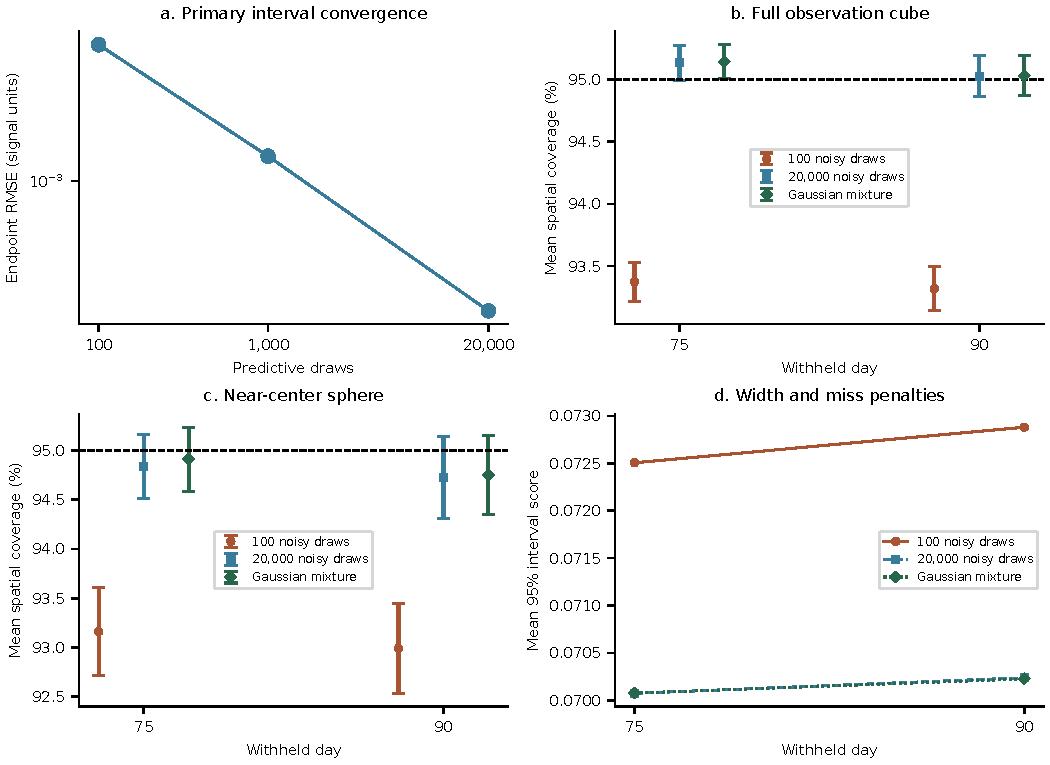
\includegraphics[width=\textwidth]{figures/pat16_prediction_validation.pdf}
\caption{Improved PAT16 pointwise 95\% prediction intervals. (a) Primary endpoint RMSE relative to Gaussian-mixture quantiles, over both tails, withheld days and all observation voxels; 100 draws use the legacy construction, while 1,000/20,000 draws resample bootstrap trajectories. (b,c) Mean spatial coverage across \PPTrials{} fresh datasets, with dataset-level Monte Carlo 95\% limits; the dashed line is nominal coverage. (d) Mean full-cube proper interval score, penalizing width and misses. Each repetition independently refits the early data and 100 bootstrap datasets; future noise is independent of training and resampling. Gaussian integration removes predictive noise sampling error, while uncertainty from finite bootstrap fits and the fixed model remains.}\label{fig:pat16_prediction_validation}
\end{figure}

The noise-free matched-model fit recovered all four generating values with maximum relative error \PRMatchedError{}; this is a matched-discretization implementation check. Fitting noise-free finer-time signals shifted WM diffusion, GM diffusion, proliferation and anisotropy by $\PRWhiteTemporalShift\%$, $\PRGrayTemporalShift\%$, $\PRRhoTemporalShift\%$ and $\PRRatioTemporalShift\%$, respectively. Thus the largest temporal-mismatch shift was \PRTemporalMaxShift\%. These deterministic shifts are outside the sampling-interval construction. The check retained the spatial anatomy and stencil and cannot establish spatial convergence. Time-zero-only inference was correctly rejected. Tests also rejected four-parameter fitting without directional information or with only one tissue class. Conditional numerical recovery and synthetic forecasting do not validate the patient observation model or biological migration anisotropy.

\begin{figure}[p]
\centering
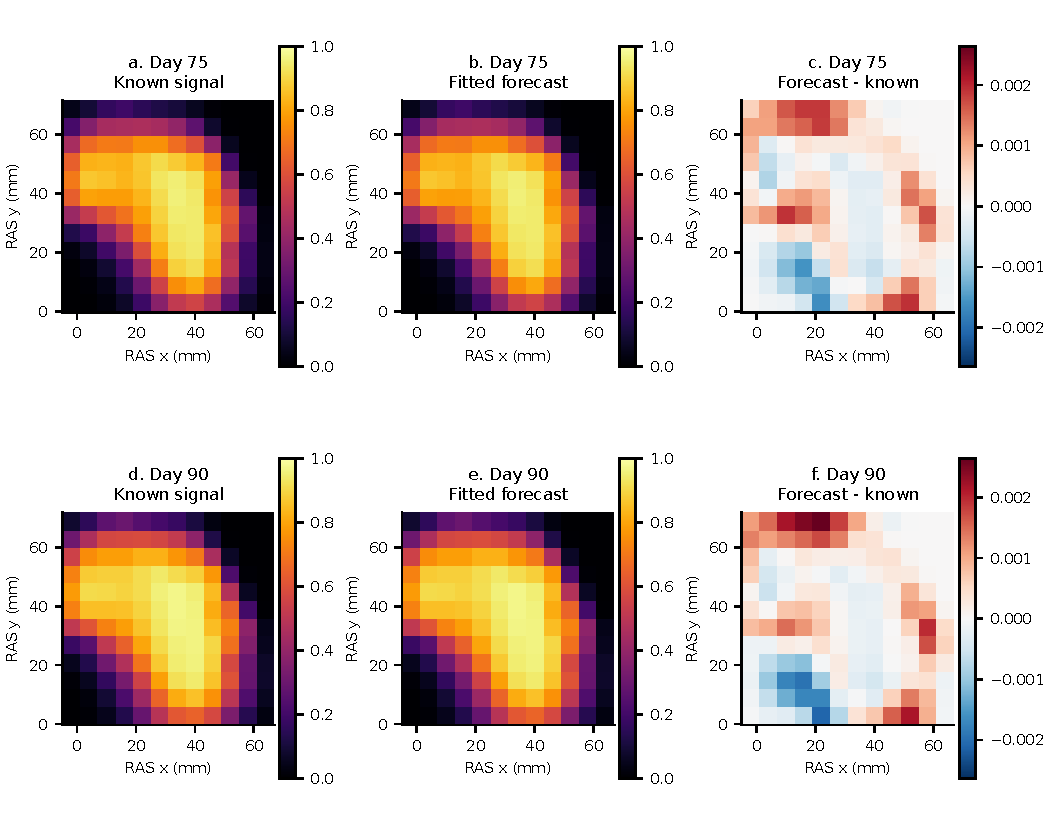
\includegraphics[width=\textwidth]{figures/pat16_recovery_forecast.pdf}
\caption{PAT16 withheld day-75 (top) and day-90 (bottom) noise-free signals on the central observation plane, RAS $z=\PRProfileZ$ mm. Left: known synthetic signal. Middle: the forecast calibrated only at days 20/40/60. Right: fitted minus known signal, with one shared symmetric residual range retaining all displayed errors. The known and fitted signals share a $0$--$1$ scale. Each pixel approximates a 6 mm cube average after Gaussian blur with 2 mm standard deviation; these are synthetic signals, not patient MRI intensities or a fine-grid tumor-density slice. Pointwise interval behavior is shown in Figure~\ref{fig:pat16_recovery}d and Table~\ref{tab:pat16_recovery_forecast}.}\label{fig:pat16_recovery_forecast}
\end{figure}
\FloatBarrier


\section{Discussion}
\subsection{Interpretation and scope of the extension}
The principal result is a separation between simulated burden and threshold-defined extent. With identical assigned migration and growth parameters, oxygen feedback lowered viable density in the interior while leaving the lower-density boundary comparatively similar. Well-oxygenated regions retain Fisher--KPP-like growth, whereas the interior experiences inhibited births and, at sufficiently low oxygen, death transfer. The ablations show that burden-dependent supply suppression dominates the overall effect for this parameter set. The numerical comparison establishes how the selected equations behave; it does not establish that they predict glioma better than Fisher--KPP. Predictive model selection requires fitting each candidate to the same calibration observations and comparing their withheld-data predictions.

The extension is deliberately small, but its state interpretation matters. Immobile $z$ with zero clearance accumulates historical cell loss, while viable cells can diffuse into the same locations. The equations therefore allow $c+z>K$ and $z>K$ locally. A normalized necrotic volume fraction should not be inferred from $z/K$. The observed grid sensitivity reinforces this limitation. If physical packing, tissue displacement or a necrotic cavity becomes a target, a volume-fraction, mechanical or poromechanical formulation would be a different model requiring additional parameters and observations. Recent MRI-informed poromechanical forecasting and sequential biomechanical model-selection studies provide relevant alternatives, but the cited 2026 records are preprints and concern distinct preclinical datasets \citep{andaloussi2026,noman2026}. They do not validate the present closure.

\subsection{What the synthetic recovery establishes}
The two recovery experiments provide a staged inference test: homogeneous diffusion/proliferation and then separate white-/gray-matter diffusion with shared proliferation were estimated from noisy, low-resolution signals. Both include local and bootstrap intervals, independent noise trials and withheld future scans. The homogeneous generator used a finer mesh and time step than inversion. The primary BrainWeb generator instead shared the spatial grid while refining time; its separate anatomy/grid stress test exposes a limitation of that favorable design. Neither experiment removes shared biological, initialization or imaging assumptions, and neither estimates coupled oxygen--necrosis mechanisms from structural MRI.

The homogeneous known rates lay within both interval constructions. In the BrainWeb primary realization, the true proliferation rate narrowly missed both 95\% intervals, while both diffusion rates were contained. Retaining that outcome is essential: a nominal confidence level does not imply containment in every realized dataset. Independent local-interval coverage of \BWWhiteCoverage/\BWTrials{}, \BWGrayCoverage/\BWTrials{} and \BWRhoCoverage/\BWTrials{} had broad binomial uncertainty. These observations do not establish bootstrap coverage, global identifiability or calibration across patients. The weaker relative precision of gray-matter diffusion and its dependence on white-matter diffusion argue for propagating the joint rate uncertainty. Separate tissue rates were estimable here without fixing their ratio, but that conclusion depends on this known seed, informative tissue exposure and observation schedule. Relaxing initialization and calibration may expose stronger confounding \citep{hiremath2025}.

The anatomy test identifies a distinct source of uncertainty. Noise-free 2 mm signals fitted with the 3 mm model shifted gray-matter diffusion by +\BWGrayStressShift\%, despite day-90 observation discrepancy remaining below the noise standard deviation. Many measurements can make sampling intervals narrow while systematic representation error persists. This shift combines tissue-boundary resampling, mesh, seed sampling and discrete imaging; it is not a measured biological change, a pure spatial-order result or an estimated segmentation-error distribution. The primary bootstrap and local covariance keep these quantities fixed and cannot quantify this effect. Inference should therefore compare multiple anatomically consistent resolutions and propagate plausible label/registration variations before interpreting tissue-rate differences biologically.

Forecast assessment also needs spatial qualification. In BrainWeb, day-90 prediction intervals contained 94.2\% of full-FOV measurements but 89.2\% near the seed. Background-inclusive summaries alone can conceal local mismatch. Mean-signal confidence bands and new-measurement prediction bands answer different questions; neither provides simultaneous image coverage here. These frequentist conditional intervals are not Bayesian posteriors or estimates of clinical variability. Next studies should vary seed location, tissue-rate contrast and scan timing, and introduce unknown age, seed shape, capacity, calibration, correlated noise and structural mismatch. A broader bootstrap-coverage audit remains separate work.

\subsection{What measurements could identify parameters?}
A practical first stage would estimate a limited growth--migration subset from serial, registered MRI, while jointly assessing initialization and whether separate tissue migration rates are supported. A constrained tissue ratio or an external prior may be needed when the measurements do not separate those rates; the conditional BrainWeb example does not establish that this restriction can be removed in patients. In a homogeneous, isotropic Fisher--KPP medium, the asymptotic minimal front speed is $v=2\sqrt{D\rho}$ and the front length scale is proportional to $L=\sqrt{D/\rho}$. These relations explain why growth velocity and spatial spread offer complementary information. They are not identities for a finite, heterogeneous brain with an unknown initial state. One snapshot with unknown tumor age generally cannot separate all dimensional rates. Recent single-scan inference methods introduce model and scaling assumptions \citep{zhang2025}; a 2026 simulated-biopsy preprint similarly distinguishes information about infiltration length from information about growth speed \citep{hofmann2026}.

\begin{table}[p]
\centering\small
\caption{Proposed measurement and prior strategy. These are candidate information sources, not measurements acquired or estimates obtained in this study. Each modality requires its own observation operator and uncertainty model.}\label{tab:measurements}
\begin{tabularx}{\textwidth}{p{0.17\textwidth}YY}
\toprule Quantity & Potential information & Restriction or prior needed\\\midrule
$c(0)$, $D$, $\rho$ & Serial T1/T2/FLAIR, diffusion-weighted and quantitative MRI; registered anatomy & Joint initialization uncertainty; estimate a small parameter subset; constrain tissue ratios. MRI water diffusion is not cell migration.\\
$K$ and cell scale & Spatially localized tumor-cell counts with tissue-volume or stereological calibration & Distinguish tumor from non-tumor cells and correct sampling/deformation; MRI alone does not fix the absolute scale.\\
$\beta$, $\alpha$ & Oxygen-sensitive imaging combined with perfusion/vascular measurements and externally calibrated uptake information & Supply and consumption are confounded; blood-flow surrogates are not the restoration coefficient itself.\\
$\ell_o$ & External transport measurements or multiscale vascular/oxygen models & Constrain externally when subvoxel; the current 1--2 mm meshes do not resolve 0.2 mm.\\
$\theta_p$, $\theta_d$, $\delta$ & Controlled oxygen-dependent growth and survival experiments; spatially matched hypoxia/viability observations & Relative-oxygen scale must be calibrated. Ki-67 is a cycling fraction, not directly a growth rate; hypoxia markers are not absolute oxygen readings.\\
$\lambda_z$ and $z$ mapping & Longitudinal necrotic-region imaging plus localized pathology & Separate formation from clearance and cell equivalents from tissue volume; a single scan cannot determine both histories.\\\bottomrule
\end{tabularx}
\end{table}

MRI-derived cell-density maps can supply more information than binary segmentations only when their calibration is defensible. ADC measures water mobility, not the effective migration coefficient $D$. Its association with cellularity is influenced by extracellular space, edema, tissue composition and necrosis \citep{eidel2016}. Nor should a FLAIR boundary automatically be treated as a fixed tumor-density contour: an MRI--histology study challenged that assumption in a single autopsy case \citep{martens2021}. In a 2025 study of image-guided biopsies, associations between MRI-derived cell-density maps and histology differed between untreated and recurrent tumors \citep{nocera2025}. The treatment context and observation mapping must therefore be part of the inference model. Biopsy coordinates, brain shift, fixation deformation, partial volume and the conversion from two-dimensional counts to cells/mm$^3$ require explicit treatment.

Oxygen introduces further observation ambiguity. The state $o$ is availability relative to a normal baseline; it is not directly oxygen extraction fraction, hemoglobin saturation or oxygen tension. Oxygen-enhanced MRI, BOLD-based measures and hypoxia PET could constrain an observation model, but their signals depend on delivery, vascular and tissue factors. A histological comparison of MRI-derived oxygen measures illustrates that an imaging surrogate cannot simply be equated with a hypoxia marker \citep{arzanforoosh2024}. The 2026 glioma habitat repeatability study is encouraging for measurement consistency, but repeatability does not establish an absolute oxygen calibration or biological specificity \citep{das2026}.

Priors are necessary where these measurements leave parameters weakly identified. Positive rates and lengths can use log-normal priors; ordered oxygen thresholds can use a transformed prior satisfying $0<\theta_d<\theta_p<1$. Hyperparameters should come from independently evaluated experiments or a defensible population model, with uncertainty reflecting transfer between systems. The working values in Table~\ref{tab:parameters} are not empirical prior means. Prior predictive checks should reveal implausible growth, oxygen depletion and accumulation above the intended interpretation of $K$. Sensitivity analysis, profile likelihoods and posterior correlations can then identify parameter combinations that the observations fail to distinguish. The 2025 identifiability/model-selection study provides a relevant framework, although its virtual-cohort chemoradiation models differ from this system \citep{hiremath2025}. A narrow posterior produced mainly by a strong prior should not be described as precise measurement-based estimation.

\subsection{Multimodal MRI and patient-specific growth forecasts}
Serial T1, gadolinium-enhanced T1 (T1-Gd), T2/FLAIR, diffusion MRI (dMRI) and functional MRI (fMRI) could constrain complementary parts of a patient-specific model (Table~\ref{tab:multimodal}). Structural images would define anatomy, abnormal tissue and the postoperative cavity; diffusion-derived microstructure could inform migration geometry and a calibrated cellularity observation model. Enhancement reflects blood--brain barrier permeability as well as tumor biology, while FLAIR abnormality can combine infiltration, edema and treatment-related changes \citep{wen2023,martens2021}. Thus neither boundary should be imposed as a universal cell-density contour. The synthetic normalized-cellularity operator used here is not an established mapping from any of these clinical sequences.

\begin{table}[tbp]
\centering\small
\caption{Proposed roles of multimodal MRI in a growth--brain digital twin. The PAT16 pilot uses existing T1, dMRI and resting-state fMRI derivatives for anatomical/directional integration and static connectivity; no patient growth rates are fitted. T1-Gd and T2/FLAIR integration remains proposed. Imaging correlates require calibration and do not directly identify every model state.}\label{tab:multimodal}
\begin{tabularx}{\textwidth}{>{\raggedright\arraybackslash}p{0.13\textwidth}YY}
\toprule Modality & Information for a proposed model & Interpretation and uncertainty\\\midrule
T1 & Anatomy, tissue compartments, displacement and resection cavity & Lesion-aware segmentation and registration; non-enhancing margins may be poorly defined.\\
T1-Gd & Enhancing compartment and permeability-related change & Enhancement is not a direct viable-cell count; surgery and treatment alter permeability.\\
T2/FLAIR & Extent of abnormal tissue and non-enhancing disease & Infiltration, edema, gliosis and treatment effects can overlap.\\
dMRI & Fiber orientations, tract architecture and diffusion-derived microstructure & Water diffusion is not cell migration; ADC-to-cellularity calibration is context dependent.\\
Resting-state fMRI & Functional connectivity and hemodynamic constraints for neural-network models & BOLD can be altered by neurovascular uncoupling; a short time series does not measure longitudinal tumor growth.\\\bottomrule
\end{tabularx}
\end{table}

The PAT16 pilot implements positive-definite, trace-matched white-matter migration tensors informed by dMRI orientations (Equation~\eqref{eq:pat16_tensor}). Parallel and transverse migration scales, and their relation to gray-matter migration, would remain parameters or externally constrained quantities; the measured water-diffusion tensor must not be substituted numerically for tumor-cell migration. Crossing fibers, edema, tract displacement and loss introduce uncertainty in the directional information itself. The scalar implementation remains a matched reference in the pilot; predictive patient comparison would require separate calibration of both variants. The anatomy sensitivity observed here argues for evaluating plausible segmentations, registration transforms and directional reconstructions jointly with rate uncertainty before attributing a fitted difference to tumor biology.

More MRI contrasts do not automatically identify the oxygen--necrosis subsystem. Perfusion measurements may help constrain delivery, while dedicated oxygen-sensitive MRI or hypoxia PET may constrain a calibrated relation to $o$; ordinary resting-state BOLD is not a tissue oxygen-concentration measurement. The 2026 repeatability work used a dedicated multiparametric protocol in a murine glioma model, rather than validating oxygen estimates from routine human fMRI \citep{das2026}. Likewise, a postoperative cavity or a radiological necrotic region cannot be equated with the accumulated cell equivalents $z$. Observation models may need additional edema, vascular or treatment-injury quantities that are absent from the present equations.

\subsection{Connecting growth, brain networks and functional outcomes}
Growth forecasts could provide the evolving lesion state for a brain digital twin. Previous studies used individual structural connectomes and The Virtual Brain to model functional connectivity in tumor patients and after resection \citep{aerts2018,aerts2020}. The related Finse 2026 repository demonstrates a T1/dMRI/resting-state-fMRI workflow linking anatomy, biomechanics, connectivity, neural dynamics and cognitive outcomes in one example, sub-PAT16 \citep{lundervold2026twin}. The present PAT16 pilot reads its processed MRI derivatives and recomputes static functional connectivity, adding a conditional migration comparison. It does not couple growth to mechanics, evolving structural connectivity or neural dynamics; those remain proposed extensions.

The underlying Brain Tumor Connectomics (BTC) data comprise 11 glioma patients, 14 meningioma patients and 11 controls before surgery, with postoperative data available for 7, 12 and 10 participants, respectively, around six months later \citep{aerts2022}. Gliomas and meningiomas should not be pooled under the same infiltrative growth law. The linked prototype supplies T1, dMRI and resting-state fMRI; T1-Gd, T2 and FLAIR would be additions. A preoperative/six-month-postoperative pair combines resection, recovery and any intervening treatment with disease evolution. It cannot be interpreted as an untreated growth interval or independently determine all migration, proliferation and response parameters. Lesion-aware registration must distinguish removed tissue from displacement; a cavity-crossing deformation is not a measured growth trajectory. Serial clinical tumor MRI, recorded treatment timing, molecular diagnosis and an explicit residual-disease state would be needed for a defensible growth-inference study.

A staged integration would first propagate ensembles of plausible tumor states through mechanics and tract-involvement models, then map these changes to structural connectivity and neural dynamics. Both direct infiltration and tissue displacement would be candidate causes of altered connectivity, with distinct parameters and observations. Resting-state fMRI would constrain the functional/hemodynamic component, while later functional measurements and cognitive scores would test its forecasts. Tumor growth over days or months and BOLD fluctuations over minutes are different time scales. Neurovascular uncoupling can produce apparent loss of functional connectivity without corresponding loss of neuronal function \citep{sun2020}; weak BOLD must therefore not be treated as proof that tissue is functionally expendable. Fitting a connectivity matrix and evaluating agreement with that same matrix is calibration, not independent validation of functional prognosis.

Bidirectional neuron--glioma coupling is a further hypothesis. Human glioblastoma work combining electrophysiology, localized tissue sampling and experimental models provides evidence for tumor--neural circuit interactions \citep{krishna2023}. It does not establish a transferable relation between resting-state BOLD amplitude or connectivity and proliferation rate, particularly across glioma subtypes. An activity-dependent growth term would require its own observation mapping, identifiable coupling parameters and independent longitudinal or perturbation evidence. Initial integration should assess functional consequences of growth before attempting to infer this feedback from sparse imaging.

For treatment evaluation, an integrated model could compare resection or radiation scenarios in terms of both residual/infiltrative burden and predicted tract, network and cognitive consequences. A next PAT16 study could extend the static overlays to conditional network effects using the observed resection and anatomical uncertainty, without claiming recovery of untreated growth or the unobserved outcome of alternative surgery. Later studies should compare growth-only, network-only and combined predictors on patient-level withheld outcomes; retrospective imaging or connectivity agreement does not establish benefit from changing treatment. Functional preservation would join tumor control, toxicity and deliverability as a separately validated objective.

\subsection{Interpretation of the PAT16 directional pilot}
The paired comparison isolates a transport-geometry choice under shared initialization, local mean diffusivity and proliferation, rather than estimating different patient growth rates. The broad marginal sensitivity bands overlap, while pairing reveals a negative day-90 burden difference for the recorded draws. This direction is conditional on the lesion, coefficients, interfaces and initialization. Trace matching fixes $\operatorname{tr}(\mathbf D)/3$ but does not impose equal spatial spreading in a bounded heterogeneous domain. Diffusion conserves mass; its redistribution changes local saturation and therefore integrated logistic births. The anisotropic calculation contains no cell-killing term, and the smaller burden is not evidence of a therapeutic effect or universally slower glioma growth. Regional redistribution can also occur despite a lower global burden.

The pilot moves beyond a healthy anatomical phantom by using a measured lesion, tissue maps and tract axes, but the state-to-image link remains assumed: a lesion mask is neither a measured cellularity field nor a calibrated MRI detection contour. A 3 mm staircase interface and the treatment of 603 lesion/CSF-classified voxels influence the transport graph. The small time-step difference and analytical tensor tests do not establish spatial convergence on this anatomy. DTI cannot resolve crossing fibers; the existing multi-shell tensor fit, FA eligibility rule, segmentation and registration require further assessment. A global 3-degree direction perturbation is a limited sensitivity probe, not a registration-error posterior. The 32-draw, independently specified ensemble omits correlated and structural uncertainty and cannot support calibrated patient risk estimates.

The static fMRI overlays locate simulated tissue involvement relative to measured correlations. They demonstrate coordinate integration and offer hypotheses for later network experiments, while regional mean density remains an anatomical overlap measure. FC edges are not axonal pathways, and projecting ROI centers through a slice slab does not locate a tract on that plane. Motion, atlas mismatch and neurovascular uncoupling affect the measured FC. Independent longitudinal connectivity and cognitive measurements, with explicit neural and hemodynamic models, are required before interpreting tumor overlap as functional impairment.

\subsection{Uncertainty quantification and informative measurements}
The positive rate correlation and forecast ensembles in the synthetic experiment illustrate why parameter estimation should quantify joint uncertainty rather than supply a single best fit. Beyond the conditional frequentist analysis performed here, a Bayesian analysis could combine independently justified priors with an observation likelihood accounting for imaging noise and spatial correlation. Hierarchical population priors could support patients with sparse imaging, provided the population model is learned within training data. Uncertain initialization, registration and segmentation should be included as nuisance quantities or evaluated through repeated analyses. Strong posterior correlations and sensitivity to alternative priors would indicate which rates or combinations remain poorly constrained.

Forecast ensembles should propagate these uncertainties into viable-burden intervals, infiltration maps and oxygen/necrosis predictions. Measurement uncertainty, numerical error and model inadequacy require separate assessment: a narrow conditional posterior does not account automatically for a wrong oxygen closure or unresolved spatial gradients. Competing Fisher--KPP and coupled formulations should be evaluated separately on withheld observations; any model-averaging weights should be learned without those evaluation data. Posterior predictive checks, interval coverage and width, and sensitivity to the observation operator should accompany point-error metrics.

Pash et al. developed a scalable Bayesian reaction--diffusion framework using longitudinal imaging and investigated imaging frequency and experimental design \citep{pash2026}. This provides a methodological reference for the proposed inference workflow, not validation of the present oxygen--necrosis extension. Once uncertainty is calibrated, candidate scan times or additional modalities could be ranked by their expected reduction in forecast uncertainty or their expected value for distinguishing treatment options. Additional measurements are useful when they resolve a consequential ambiguity, rather than merely increasing the number of fitted parameters.

\subsection{A validation pathway with independent targets}
Validation must be tied to a specified observable, population and prediction horizon. Five complementary stages are appropriate here.
\begin{enumerate}
\item \textbf{Verify the solver.} Check conservation, positivity, analytical limits, solver tolerances and time/space refinement. These checks address mathematical implementation. The present unresolved oxygen length and necrotic peak require further spatial assessment before local quantitative claims.
\item \textbf{Extend synthetic recovery.} The homogeneous and BrainWeb experiments supply controlled two- and three-rate recovery and withheld-scan checks. Broaden them across seed locations, rates, anatomy representations and scan schedules, and add unknown initialization, correlated noise, registration error and observation-model mismatch. Use a different mesh, solver or observation formulation to reduce the inverse crime of fitting data generated by the identical numerical pipeline. Synthetic success does not establish biological adequacy; earlier MRI-constrained reaction--diffusion work demonstrated the importance of separating synthetic recovery from in vivo forecasting \citep{hormuth2015}.
\item \textbf{Forecast withheld observations.} Fit early observations, freeze the calibration and measurement mapping, and predict later scans over a declared horizon. Compare separately calibrated M0, M1 and M2 with a simple growth baseline. Treated tumors require explicit treatment terms or a justified untreated interval. Updating with each new scan is sequential assimilation, a different evaluation from a frozen forecast. The 2025 assimilation study illustrates the distinction in high-grade glioma during chemoradiation \citep{miniere2025}.
\item \textbf{Check latent fields independently.} Reserve spatially localized cell counts, viable/necrotic histology and oxygen-related observations for evaluation rather than using all samples for calibration. Report localization and measurement uncertainty. A successful volume forecast alone does not validate $o$, $z$ or the death mechanism. Controlled preclinical oxygen or perfusion perturbations would provide stronger tests of the proposed feedback than morphology alone.
\item \textbf{Evaluate transportability.} Apply a fixed analysis and prior strategy to an external cohort, with any permitted patient-specific calibration specified in advance. Group splits by patient and, where relevant, site and treatment status. Prospective clinical utility is a subsequent question, beyond retrospective image agreement.
\end{enumerate}

Evaluation should include volume errors, surface distances and overlap, together with quantitative field errors where calibrated measurements exist. Report predictive interval coverage and width, not only point accuracy. Repeated biopsies within a patient and spatially correlated voxels are not independent replicates; patient-level or hierarchical analyses should reflect this dependence. The 2025 biopsy-validation study is a useful example of independent tissue evaluation and context-dependent agreement \citep{nocera2025}. An accurate forecast can coexist with non-unique physiological parameters, while an identifiable model can still have the wrong biology. Both prediction and parameter interpretation must be assessed.

Clinical validation should subsequently use a prespecified population, prediction horizon and analysis, with external testing before prospective, blinded forecasting. Imaging endpoints should account for treatment effects and pseudoprogression using a defined response-assessment framework such as RANO 2.0 \citep{wen2023}. Agreement with a later MRI or recurrence location is evidence about prediction under the observed treatment; it does not establish the outcome under an alternative treatment. Demonstrating clinical utility would require prospective comparative evaluation of decisions and, ultimately, controlled trials assessing survival, neurological function, quality of life and toxicity.

\subsection{Treatment evaluation and candidate strategies}
The present simulations suggest why treatment evaluation should consider viable burden and spatial infiltration together: similar threshold-defined volumes can conceal different modeled interiors. Their difference is not a treatment effect, because no therapy was simulated. Extending the framework would require an explicit resection geometry and residual disease state, spatially delivered radiation and drug exposure/response terms. Surgery may also change anatomy and perfusion, requiring updated transport and observation models. Natural growth and treatment-response parameters should be estimated jointly from appropriately timed observations, or constrained independently when they cannot be separated.

An oxygen-dependent radiation-survival model could test the consequences of hypoxia and reoxygenation between fractions, but the relative availability $o$ first needs a calibrated connection to the relevant radiobiology. Neither $c$ nor $z$ currently represents a measured clonogenic population or radiation-induced normal-tissue injury. Computing a tumor-control probability would require additional assumptions about clonogenic fraction and survival; evaluating toxicity would require a separate normal-tissue model. Treatment-related necrosis and imaging changes must be distinguished from spontaneous hypoxic loss. These additions are proposed mechanisms requiring independent experiments, not interpretations already supported by the three simulated fields.

Recent studies illustrate complementary evaluation targets. Balcerak et al. evaluated imaging- and physics-informed infiltration estimates against subsequent recurrence in a dataset of 152 glioblastoma patients \citep{balcerak2025}. H\"ager et al. examined model-informed target delineation and voxel-based dose planning in three cases, demonstrating planning feasibility while identifying difficulties in reproducing complex dose distributions \citep{hager2026}. These retrospective prediction and planning studies do not establish a survival benefit from delivering the proposed alternatives. Earlier risk-aware radiotherapy optimization used a cohort of 100 virtual patients \citep{chaudhuri2023}, illustrating how uncertainty can inform simulated treatment comparisons without constituting a clinical trial.

A next experimental stage could use paired virtual cohorts to compare a specified standard-treatment comparator with adaptive fractionation, spatial dose painting, hypoxia-modifying combinations and alternative drug/radiation sequences. Each candidate would require an explicit mechanism and independently constrained response parameters. Comparisons should use matched dose/resource constraints, assess normal-brain exposure and delivery feasibility, and test whether a favorable ranking persists across parameter and model uncertainty. Adaptive policies must use only observations available at the decision time. Outcomes could include viable burden, spatial recurrence and time to a prespecified progression criterion; a survival prediction would require a separately validated link to that endpoint. Controlled preclinical oxygen/perfusion perturbations could test the proposed feedback before patient translation. Virtual cohorts should prioritize experimentally testable hypotheses and informative measurements; they cannot identify an effective new therapy solely from a favorable simulated result.

\subsection{Limitations and staged roadmap}
The anatomical comparison uses one healthy phantom, one seed and one primary parameter set. The ablations and refinement runs are not a population analysis. The recovery experiments vary noise around two fixed states, including one BrainWeb seed; they do not sample between-patient heterogeneity or calibrate the dense-seed oxygen--necrosis comparison. The 3 mm primary BrainWeb fit shares tissue geometry with its generator, and one 2 mm sensitivity example is not a distributional audit of anatomy uncertainty. Scalar migration in the BrainWeb comparison omits fiber orientation; the separate single-patient pilot adds DTI-informed transport but no spatial convergence or patient growth validation. No displacement, edema, vascular evolution, immune interactions, phenotype switching or therapy is modeled. Quasi-steady oxygen identifies effective coefficient groups rather than absolute oxygen equilibration rates. Minimum oxygen and necrotic accumulation are under-resolved, and zero clearance accentuates accumulation. Finer simulation grids do not create additional measurement information.

The following sequence makes the roadmap concrete, building on the numerical comparisons and conditional synthetic recovery reported here.
\begin{enumerate}
\item \textbf{Establish an estimable MRI model.} Resolve the coupled-model numerical limitations and calibrate sequence-specific T1/T1-Gd/T2/FLAIR and diffusion observation operators. Extend two- and three-rate recovery across uncertain initialization and anatomy and extend the PAT16 directional comparison to separately fitted isotropic and anisotropic models. Add oxygen/death parameters only when independent measurements or justified priors constrain them.
\item \textbf{Broaden uncertainty assessment.} Propagate initialization, registration, tissue-label, tract-direction and imaging-model uncertainty, explicitly testing the anatomy sensitivity found here. Audit coverage, bootstrap calibration and prior sensitivity while separating numerical and model errors.
\item \textbf{Demonstrate external forecasting.} Fit early scans and predict withheld later observations with separately calibrated variants and simple baselines. Distinguish untreated growth from postoperative/treatment response, then test an external cohort and independent spatial biological targets.
\item \textbf{Connect growth to functional outcomes.} Build on the PAT16 anatomical integration and static overlays, then test mechanics/tract/connectome couplings and neural dynamics against withheld fMRI and cognitive outcomes across patients. Preserve a separate hemodynamic observation model and test whether integration improves on growth-only and network-only baselines.
\item \textbf{Evaluate treatment hypotheses.} Implement and verify treatment and normal-tissue effects, calibrate their response parameters, and compare feasible strategies with matched treatment constraints in virtual cohorts and controlled experiments. Include functional preservation and informative imaging schedules.
\item \textbf{Test clinical utility.} Evaluate prospective, blinded forecasts before controlled trials of model-guided care, with prespecified patient benefit and harm endpoints.
\end{enumerate}
Add complexity only to address predictive discrepancies supported by independent observations. Each stage requires its own evidence.

\subsection{Conclusion}
A minimal oxygen--necrosis extension can be implemented alongside Fisher--KPP within the same anatomical and interactive workflow. Under the assigned conditions, the extension reduced viable burden much more than low-threshold extent, largely through growth inhibition. Its localized necrotic predictions were sensitive to grid spacing and cannot be interpreted as validated tissue fractions. Staged synthetic experiments estimated homogeneous and tissue-specific baseline rates with conditional uncertainty and withheld forecasts. A proliferation interval miss was retained, and anatomy/grid changes produced a material gray-matter rate shift that noise-based intervals do not capture. The PAT16 pilot additionally demonstrates trace-matched directional growth and static MRI/network integration under assumed parameter distributions. Together, the code, recorded experiments and manuscript provide a tested starting point for measurement-based inference and staged validation; patient calibration and independent biological evaluation remain necessary.

\subsection*{Code, data and supplementary material}
The manuscript, source code, interactive Jupyter notebooks, recorded simulations, synthetic recovery observations and synchronized visualizations are available at \url{https://github.com/arvidl/brainweb_fisher_kpp}. The manuscript project includes LaTeX/BibTeX sources, simulation and figure-generation scripts, machine-readable experiment records, source and data hashes, and numerical-test results. Repository history and the recorded source hashes identify the implementation used for this study. An immutable release identifier and archival DOI should accompany a submitted version when available. BrainWeb attribution and source records are retained separately from the software.
\subsection*{Study scope and declarations}
All experiments are computer simulations on anatomical or homogeneous phantoms. No patient measurements, new human sampling or new animal experiments were used. Parameter recovery used synthetic measurements only; patient calibration and external biological validation remain proposed work. Authorship, affiliations, funding, competing interests, contributions and any required AI-use declaration must be finalized before journal submission.
\clearpage
\appendix
\section{Anatomical data and initialization}\label{app:data}
The files are \path{data/t1_icbm_normal_1mm_pn0_rf0.nii.gz} and \path{data/phantom_1.0mm_normal_crisp.nii.gz}. The former is the BrainWeb T1 alias with 1 mm spacing, zero added noise and zero intensity nonuniformity; the latter is the matching original normal crisp phantom, converted from MINC to NIfTI. These are not the separate BrainWeb 20-subject anatomical models. Both native arrays have shape $181\times217\times181$ and the same RAS+ affine
\begin{equation}
 A=\begin{pmatrix}1&0&0&-90\\0&1&0&-126\\0&0&1&-72\\0&0&0&1\end{pmatrix}.
\end{equation}
Native gray- and white-matter voxel counts are 902,912 and 674,777. Tissue labels 2, 3 and 8 define the active domain; label 8 uses gray-matter coefficients. CSF is label 1 and is excluded. No tumor is present in the source images. T1 intensities are divided by their 99.8th percentile and clipped for background display only; they do not determine transport or growth coefficients. At 2 mm the affine diagonal is $(2,2,2,1)$ with the same translation, and array shape is $91\times109\times91$.

The SHA-256 checksums of the bundled compressed files are:
\begin{quote}\footnotesize
T1: \nolinkurl{aa40262b2702653188fd51bdec844a393b825650fe1155a84d8606f5dfd99eb3}\\
Labels: \nolinkurl{afdff78fc1b06ad7c7d8216cf96be737a1450ef5b6abf27eb732c0bf8b66fac0}.
\end{quote}
The manifest retains official aliases and source URLs. Regenerating a MINC-to-NIfTI conversion can change compression/header encoding and therefore file hashes; a replacement requires an explicit voxel/affine comparison and updated manifest. BrainWeb attribution and terms remain applicable to these data.

For $\bm{x}_0=(-30,25,30)$ mm and $\sigma_k=6$ mm, let $r^2=\sum_{k=1}^{3}[(x_k-x_{0k})/\sigma_k]^2$. The initialization is
\begin{equation}
 c(\bm{x},0)=80{,}000\exp(-r^2/2)\,\mathbf{1}_{\{r^2\leq9\}}\,\mathbf{1}_{\Omega}(\bm{x}),\qquad z(\bm{x},0)=0 .
\end{equation}
Oxygen is initialized by the elliptic solve. The physical center is retained when grids change. The nearest saved slice indices on the 2 mm grid are $(30,76,51)$, corresponding to RAS $(-30,26,30)$ mm: the saved coronal plane is at 26 mm, rather than the off-grid 25 mm seed coordinate. Figure~\ref{fig:orthogonal} supplies orthogonal views of the same fields as Figure~\ref{fig:fields}.

\begin{figure}[p]
\centering
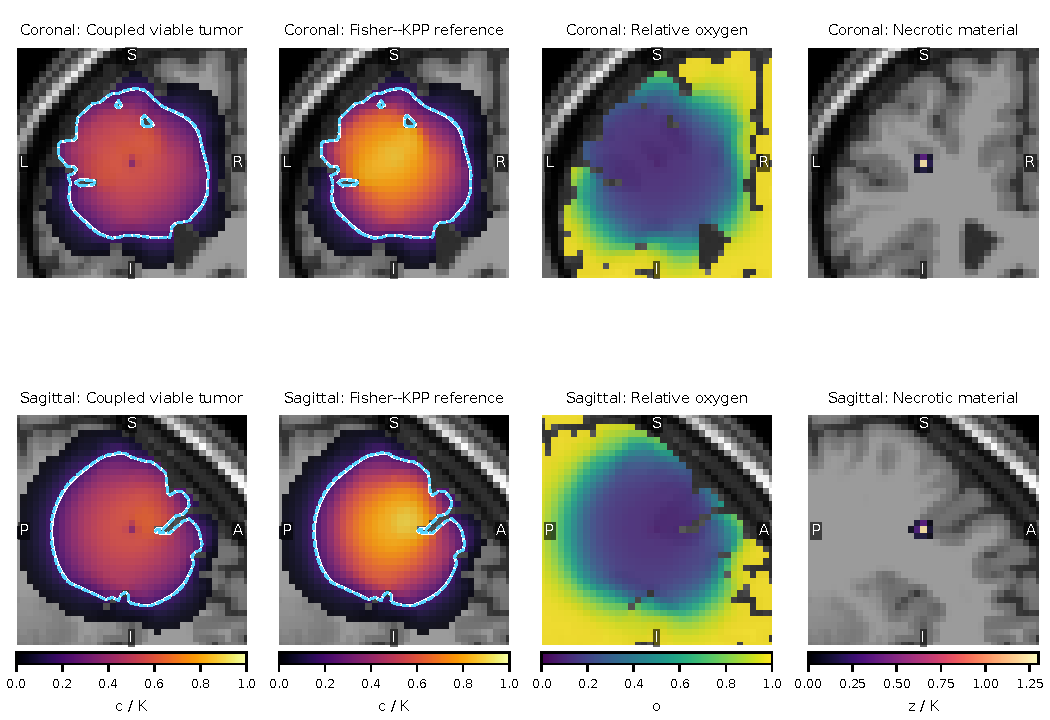
\includegraphics[width=\textwidth]{figures/orthogonal_fields.pdf}
\caption{Orthogonal day-90 comparisons through the saved seed planes: coronal $y=26$ mm (top) and sagittal $x=-30$ mm (bottom). Each panel spans $72\times72$ mm with native 2 mm pixels. Columns show coupled viable density, the matched Fisher--KPP reference, relative oxygen and necrotic material. The viable and reference scales are identical, and the necrotic scale extends to 1.3. White solid and cyan dashed contours indicate the respective $c/K=0.2$ boundaries.}\label{fig:orthogonal}
\end{figure}

\section{Numerical implementation and verification}\label{app:numerics}
\subsection{Conservative transport and reaction splitting}
For neighboring active cells $i,j$ on a Cartesian grid of spacing $h$, use the harmonic face coefficient
\begin{equation}
 D_{ij}=\begin{cases}2D_iD_j/(D_i+D_j),&D_i+D_j>0,\\0,&\text{otherwise},\end{cases}\qquad
 w_{ij}=D_{ij}/h^2 .
\end{equation}
Faces leaving the active domain are assigned zero weight, as are external volume faces. A cell-transport step is
\begin{equation}
 c_i^*=c_i^n+\Delta t\sum_{j\in\mathcal N(i)}w_{ij}(c_j^n-c_i^n),\qquad
 \Delta t\leq\frac{0.9}{\max_i\sum_j w_{ij}} .
\end{equation}
Symmetric fluxes conserve total cell count under pure diffusion. The step bound is sufficient for nonnegative explicit updates. Faces are stored without periodic wrapping; no density clipping is applied. Requested steps are subdivided as needed, and steps end at the exact saved output times.

For M0, the reaction following diffusion is the exact logistic flow
\begin{equation}
 c_i^{n+1}=\frac{c_i^*}{\exp(-\rho_i\Delta t)+(c_i^*/K_i)[1-\exp(-\rho_i\Delta t)]}.
\end{equation}
For M2, freeze oxygen at $o^n$ and necrosis at $z^n$ during birth. Set $F_i=K_i-z_i^n$. If $F_i>0$ and $c_i^*<F_i$, use
\begin{equation}
 r_i=\rho_i g(o_i^n)F_i/K_i,\qquad
 c_i^b=\frac{c_i^*}{\exp(-r_i\Delta t)+(c_i^*/F_i)[1-\exp(-r_i\Delta t)]}.
\end{equation}
Otherwise $c_i^b=c_i^*$. With $q_i=\delta h(o_i^n)$, the subsequent death/clearance step is
\begin{equation}
 L_i=c_i^b[1-\exp(-q_i\Delta t)],\quad
 c_i^{n+1}=c_i^b-L_i,\quad
 z_i^{n+1}=(z_i^n+L_i)\exp(-\lambda_z\Delta t).
\end{equation}
The same $L_i$ leaves $c$ and enters $z$, preserving cell equivalents when clearance is zero. Exact frozen-coefficient substeps do not make the full coupled update exact: diffusion, birth, death and clearance are Lie-split, and oxygen is lagged. The complete method is first order in time. The centered spatial stencil has second-order consistency in smooth regions, without a global spatial-order claim at sharp tissue boundaries. Tumor and necrosis arrays use float32 and compiled Numba CPU kernels.

\subsection{Quasi-steady oxygen solve}
Let $L_h$ be the unit-diffusivity no-flux Laplacian on the active voxel graph, $u=c/K$, and $p_i=[1+\alpha(c_i+z_i)/K_i]^{-1}$. After initialization and each tumor update, solve
\begin{equation}
 \left[-\ell_o^2L_h+\operatorname{diag}(p+\beta u)\right]\bm{o}=\bm{p}.
\end{equation}
The positive reaction diagonal makes this system symmetric positive definite, including disconnected tissue components. Matrix-free conjugate gradients use float64 arithmetic, the previous oxygen state as the initial guess and a Jacobi preconditioner. The relative residual tolerance is $10^{-7}$, with a 200-iteration maximum per solve. Nonconvergence or oxygen-bound failure raises an error. The zero-uptake and zero-diffusion limits have direct solutions. Stored oxygen is float32. Outside-domain zeros are excluded-domain sentinels and are excluded from oxygen statistics and overlays.

The primary M2 run required 361 solves and 873 total conjugate-gradient iterations; the largest recorded relative residual was below $10^{-7}$. This residual measures algebraic solution accuracy, not accuracy of the continuum approximation on the chosen grid.

\subsection{Recorded checks and refinement comparisons}
The \TestCount{}-test suite includes exact logistic growth; reflecting-boundary diffusion modes; heterogeneous-flux conservation; impermeable interfaces and no wrapping; positivity and unsafe-step rejection; parameter checks; exact output times; data affine/tissue checks; uniform and nonuniform oxygen solutions; oxygen barriers; exact death transfer and clearance; occupied-capacity behavior; Fisher--KPP recovery; live-plus-dead balance; coupled temporal refinement against an independent Runge--Kutta calculation; failed-solver reporting; rendering; and replay compatibility. Test results are stored in \texttt{paper/data/pytest.xml}. Notebook smoke checks and media review are separate interface checks.

For field $v$, final relative $L^2$ differences are $\|v_{\Delta t}-v_{0.0625}\|_2/\|v_{0.0625}\|_2$ on the same 2 mm grid (Table~\ref{tab:errors}). The denominator is nonzero in these cases. These are finite-reference differences, not rigorous continuum error bounds. The 1 mm assessment is reported in Table~\ref{tab:refinement}; because the tissue labels also change under resampling, it is not used to infer spatial order.

\begin{table}[tbp]
\centering\small
\caption{Final relative $L^2$ differences (percent) against the 0.0625-day M2 calculation on the 2 mm grid.}\label{tab:errors}
\begin{tabular}{rrrr}
\toprule $\Delta t$ (days) & Viable tumor & Oxygen & Necrotic material\\\midrule
\ErrorRows
\bottomrule
\end{tabular}
\end{table}

\section{Inverse formulation, priors and identifiability}\label{app:inference}
\subsection{An example estimation objective}
With the observation model in Equation~\eqref{eq:observation}, a possible maximum-a-posteriori objective for continuous approximately Gaussian observations is
\begin{align}
 (\widehat{\bm\theta},\widehat{\bm\eta})
 &=\arg\min_{\bm\theta,\bm\eta}\ \mathcal J(\bm\theta,\bm\eta),\\
 \mathcal J&=\frac12\sum_{m,j}\bm r_{mj}^{\mathsf T}\Sigma_{mj}^{-1}\bm r_{mj}
 -\log\pi(\bm\theta,\bm\eta),\qquad
 \bm r_{mj}=\mathcal H_m[\bm s_{\bm\theta}(t_j);\bm\eta_m]-\bm y_{mj},
\end{align}
where $\bm s=(c,o,z)$ and $\Sigma$ models measurement covariance. Cross-time or cross-modality correlations require a joint likelihood rather than independent terms. Segmentations may need a probabilistic classification likelihood rather than Gaussian residuals. Registration, partial volume, scanner bias, initial fields and uncertain state-to-signal mappings should enter the likelihood or be propagated as nuisance uncertainty. Bayesian sampling can quantify uncertainty; an optimizer alone does not provide calibrated predictive intervals. No such fit was performed in this study.

\subsection{Important structural and practical ambiguities}
\begin{enumerate}
\item \textbf{Absolute cell scale.} In terms of $u=c/K$ and $w=z/K$ with uniform $K$, the normalized dynamics do not determine $K$. Scaling $(c,z,K)$ together leaves $(u,w,o)$ unchanged. An observation dependent only on normalized density cannot identify the absolute cell count without external calibration.
\item \textbf{Age and rates.} For an unknown elapsed tumor age, multiplying $D$, $\rho$, $\delta$ and $\lambda_z$ by a common factor and dividing the elapsed time by that factor leaves the autonomous state trajectory at the observation unchanged. Known longitudinal time intervals can break this particular scaling, although seed and parameter confounding may remain.
\item \textbf{Oxygen-growth coupling.} Where all observed cells remain below $\theta_p$, the birth term depends on $\rho/\theta_p$ rather than on those parameters separately, for a fixed oxygen field. Oxygen threshold calibration and observations spanning informative regimes are needed.
\item \textbf{Delivery and uptake.} Neglecting spatial oxygen transport locally gives
\begin{equation}
 o=\frac{1}{1+\beta u[1+\alpha(u+w)]}.
\end{equation}
One local state constrains an effective supply--uptake combination, not separate mechanisms. Spatially varying, calibrated oxygen observations across burdens could help, but do not guarantee recovery. An exchange length far below measurement and mesh resolution can be practically unidentifiable.
\item \textbf{Quasi-steady reduction.} If a dimensional oxygen equation is divided by a baseline restoration rate, $\ell_o^2$ and $\beta$ represent coefficient ratios. Steady observations alone cannot identify an independent absolute oxygen relaxation time removed by that reduction.
\item \textbf{Necrotic history.} For known $q=\delta h(o)$,
\begin{equation}
 z(t)=z(0)e^{-\lambda_z t}+\int_0^t q(s)c(s)e^{-\lambda_z(t-s)}\,\dd s .
\end{equation}
A single terminal necrotic measurement cannot generally separate formation history and clearance. Zero clearance is a model choice here, not an estimated absence of biological removal.
\end{enumerate}

Positive parameters can be transformed as $\log\theta_k\sim\mathcal N(\mu_k,\sigma_k^2)$, with dimensional reference units stated. For thresholds, use $\theta_p=\operatorname{logit}^{-1}(a)$ and $\theta_d=\theta_p\operatorname{logit}^{-1}(b)$. A zero-clearance component or other exact-zero ablation requires an explicit point mass or a separate model, rather than a continuous positive prior. Neither prior hyperparameters nor population distributions are supplied by the current phantom experiment.

Before a full fit, evaluate scaled observation sensitivities, their singular values, profile likelihoods and posterior dependence across plausible initial states and observation mappings. The number of voxels is not the number of independent constraints. Begin with a global migration scale and growth coefficient, restrict other quantities using external information, and add freedom only when independent observations support it. Identifiability and predictive comparison should be repeated for each candidate model and intended measurement set.

\section{Reproducibility and interactive artifacts}
\path{paper/run_experiments.py} runs the nine model/step/grid cases using \path{examples/coupled.json}, verifies the bundled data and checks that the primary viable-count trajectory matches the saved example. It records final metrics and settings in \texttt{experiments.json}, time courses in \texttt{timecourses.csv}, lossless final seed-plane fields in \texttt{day90\_planes.npz}, and provenance in \texttt{provenance.json}, all under \texttt{paper/data/}. Source hashes include the model, data loader, renderer, configuration, lockfile and experiment script. The experiments were generated before their implementation changes were committed, so provenance records working-file hashes alongside the base Git revision. The hashes identify the simulation sources independently of that earlier revision.

\texttt{paper/make\_figures.py} reads these records to generate figures, table rows and numerical macros used directly by the manuscript. The local Python environment is defined by \texttt{pyproject.toml} and \texttt{uv.lock}. A \texttt{Makefile} rebuilds the figures and PDF, with a separate target to rerun the experiments. The native and 2 mm examples are deterministic; they do not sample biological uncertainty.

\texttt{tumor\_growth\_explorer.ipynb} exposes both models; \texttt{coupled\_example.ipynb} presets the 90-day comparison. Time and RAS slices are shared across the four-field view. Live histories permit arbitrary 3D slicing, while compact replay files retain the three seed-plane histories and final full volumes. The slower comparison MP4 uses 400 frames at 20 frames/s, including a 120-frame day-90 hold; playback duration is distinct from simulated time. Synchronized movies help inspect output but are not quantitative validation. Manuscript figures retain the full computed necrotic range, unlike a display limited to $0$--$1$.

\clearpage
\bibliographystyle{unsrtnat}
\bibliography{references}
\end{document}
